\documentclass[12pt,a4paper]{article}
\usepackage[margin=2.5cm]{geometry}
\usepackage{amsmath,amssymb}
\usepackage{graphicx}
\usepackage{hyperref}
\usepackage{booktabs}
\usepackage{xcolor}
\usepackage{tikz}
\usetikzlibrary{arrows.meta,positioning}
\usepackage{caption}
\usepackage{subcaption}
\usepackage{float}
\usepackage[english]{babel}
\usepackage{microtype}
\usepackage{enumitem}
\usepackage[most]{tcolorbox}
\usepackage{array,tabularx,multirow,colortbl}
\usepackage[numbers]{natbib}

\hypersetup{colorlinks=true,linkcolor=blue!60!black,
  citecolor=green!40!black,urlcolor=orange!70!black}

\definecolor{wingreen}{HTML}{d4edda}
\definecolor{lossred}{HTML}{f8d7da}

\tcbset{
  mdpbox/.style={colback=blue!4,colframe=blue!45!black,
    fonttitle=\bfseries,boxrule=0.7pt,arc=3pt,
    left=6pt,right=6pt,top=4pt,bottom=4pt},
  findbox/.style={colback=green!4,colframe=green!45!black,
    fonttitle=\bfseries,boxrule=0.7pt,arc=3pt},
  warnbox/.style={colback=orange!4,colframe=orange!55!black,
    fonttitle=\bfseries,boxrule=0.7pt,arc=3pt}
}

\title{%
  \textbf{Reinforcement Learning for Algorithmic Trading}\\[4pt]

  \normalsize Seminar Report
}
\author{Parakh Sharma - 24B0729 \\
  \small Centre for Multidisciplinary Education\\
  \small Indian Institute of Technology Bombay
}
\date{May 2026}

\begin{document}
\maketitle

\begin{abstract}
Rule-based algorithmic trading strategies are static by design and cannot
adapt when market regimes shift. Reinforcement learning~(RL) offers a
data-driven alternative in which an agent directly optimises a risk-adjusted
reward signal. This report implements and evaluates \textbf{RecurrentPPO}
with an LSTM encoder across 12 US equities (spanning bull, bear/crash,
volatile, and sideways categories) and 5 major cryptocurrencies (BTC, ETH,
BNB, SOL, XRP). Agents are trained under two distinct regimes---a
bull-dominant window~(Period~A) and a mixed bull-bear window~(Period~B)---to
quantify how training data composition affects out-of-sample performance.

Our central finding is that \textbf{RL performance is strongly
regime-dependent and training data composition is the dominant determinant
of agent quality}. 
% Key results: COIN~(+131.6\% PPO vs $-86.2$\% B\&H),
% PYPL~(+87.3\% vs $-66.1$\%), META~(+125.0\% vs +104.4\%, Period~B),
% BNB~(+21.4\% vs +11.0\%, Sharpe 0.32 vs 0.21). In sustained bull markets,
% MACD Long/Flat and Buy~\&~Hold remain competitive. This regime-dependence
% is itself the key contribution.
\end{abstract}

\newpage\tableofcontents\newpage

\section{Introduction}

Financial markets are non-stationary and adversarial. Classical algorithmic
strategies address this by encoding human expertise into fixed rules: the
MACD crossover buys when a short EMA crosses a long EMA; Buy~\&~Hold
simply holds the asset indefinitely. These rules are interpretable and
auditable, but fixed at design time and unable to adapt when market
conditions change.

Reinforcement learning reframes the problem. Rather than specifying a rule,
we define a reward signal encoding what we actually care about---risk-adjusted
profit net of transaction costs---and let an agent discover an optimal policy
through experience. The agent learns \emph{from data} rather than from
hand-crafted heuristics.

This report makes the following contributions:
\begin{enumerate}[nosep]
  \item A complete implementation of single-asset RecurrentPPO~(LSTM)
        trading agents for signal-based trading.
  \item Systematic evaluation across \textbf{17 assets}---12 equities
        across 4 market categories and 5 cryptocurrencies---under two
        distinct training regimes.
  \item Quantitative analysis of when RL outperforms classical
        baselines and when it does not.
  \item Empirical demonstration that training data regime is more important
        than agent architecture for real-world trading performance.
\end{enumerate}

\section{Background}

\subsection{Direct Reinforcement for Trading}

The application of RL to trading was pioneered by \citet{moody2001}, who
proposed optimising the Sharpe ratio directly as the reward---a Direct
Reinforcement approach that bypasses price forecasting. Their Recurrent
Reinforcement Learning~(RRL) algorithm adjusts trading parameters to
maximise the differential Sharpe ratio. Our reward design inherits this
philosophy: the rolling Sharpe component of our reward is the online
approximation of their differential Sharpe ratio.

\subsection{Proximal Policy Optimisation}

We use PPO \citep{schulman2017} as the training algorithm. PPO optimises
the clipped surrogate objective:
\begin{equation}
  L^{\text{CLIP}}(\theta) = \mathbb{E}_t\!\left[
    \min\!\left(r_t(\theta)\hat{A}_t,\;
      \mathrm{clip}(r_t(\theta),1{-}\epsilon,1{+}\epsilon)\hat{A}_t
    \right)
  \right],\quad \epsilon=0.15,
\end{equation}
where $r_t(\theta)=\pi_\theta(a_t|s_t)/\pi_{\theta_{\rm old}}(a_t|s_t)$ and
$\hat{A}_t$ is the generalised advantage estimate. The clipping prevents
destructively large policy updates under the noisy reward signals
characteristic of financial time series.

\section{Experimental Design}

\subsection{Asset Universe}

\begin{table}[H]
\centering
\caption{Asset universe.}
\label{tab:assets}
\begin{tabular}{lll}
\toprule
\textbf{Category} & \textbf{Tickers} & \textbf{Characteristic} \\
\midrule
Bull equities     & AAPL, MSFT, GOOGL        & Sustained upward trend \\
Bear/crash        & META, PYPL, NFLX         & Major drawdowns 2021--22 \\
Volatile          & TSLA, AMD, COIN          & Sharp swings both directions \\
Sideways/mixed    & INTC, IBM, GE            & Range-bound, low momentum \\
\midrule
Cryptocurrency    & BTC, ETH, BNB, SOL, XRP  & One test period (mixed train) \\
\bottomrule
\end{tabular}
\end{table}

\subsection{Two Training Periods for Equities}

\begin{table}[H]
\centering
\caption{Training and test periods for equities.}
\label{tab:periods}
\begin{tabular}{llll}
\toprule
\textbf{Period} & \textbf{Train} & \textbf{Test} & \textbf{Regime} \\
\midrule
A & 2018-01-01\,$\to$\,2021-12-31 & 2022-01-01\,$\to$\,2023-12-31 &
  Bull train $\to$ bear+recovery test \\
B & 2019-01-01\,$\to$\,2022-06-30 & 2022-07-01\,$\to$\,2023-12-31 &
  Mixed train $\to$ recovery \\
\bottomrule
\end{tabular}
\end{table}

\noindent\textbf{Crypto}: Train 2019-01-01\,$\to$\,2022-06-30 (includes 2022 crash);
test 2022-07-01\,$\to$\,2023-12-31 (bear bottom $\to$ recovery).

\subsection{Baselines}

\textbf{Buy \& Hold}: Full allocation on day one, no rebalancing.

\textbf{MACD Crossover (Long/Flat)}: Go long when 12-day EMA crosses above
26-day EMA (signal~9); go \emph{flat} otherwise. Does \textbf{not} short---matching
realistic institutional usage.

\section{Model Architecture}

\subsection{MDP Formulation}

\begin{tcolorbox}[mdpbox,title=MDP---Single-Asset Signal Trading]
\begin{tabular}{@{}ll@{}}
\textbf{State} $s_t$ &
  20 days $\times$ 9 features + current position $\;\Rightarrow\;$ dim~181\\[3pt]
\textbf{Action} $a_t$ &
  $\{0,1,2\}\mapsto\{-1,\,0,\,+1\}$ (short, flat, long) \\[3pt]
\textbf{Reward} $r_t$ &
  $0.1\cdot\mathrm{Sharpe}_{30} + 2.0\cdot\min(\mathrm{DD}_t,0)
   + \text{direction bonus}$ \\[3pt]
\textbf{Horizon} & One decision per trading day \\
\end{tabular}
\end{tcolorbox}

The direction bonus rewards correct directional calls:
$1.0|r^{\rm asset}|$ for a correct short on a down day and
$0.8|r^{\rm asset}|$ for a correct long on an up day. Without this term,
the agent defaults to flat (zero position) to avoid the drawdown penalty---a
degenerate but locally safe policy.

\subsection{Feature Engineering}

Nine features capture trend, momentum, mean-reversion, and volatility:

\begin{table}[H]
\centering
\caption{Input features---9 per asset per day.}
\label{tab:features}
\begin{tabular}{lll}
\toprule
\textbf{Feature} & \textbf{Definition} & \textbf{Purpose} \\
\midrule
Log-return        & $\ln(P_t/P_{t-1})$                     & Today's move \\
5d momentum       & $P_t/P_{t-5}-1$, clip $\pm0.15$        & Short trend \\
15d momentum      & $P_t/P_{t-15}-1$, clip $\pm0.15$       & Medium trend \\
30d momentum      & $P_t/P_{t-30}-1$, clip $\pm0.20$       & Longer trend \\
RSI-14            & RSI normalised to $[0,1]$              & Overbought/sold \\
10d volatility    & Rolling std of log-returns             & Short regime \\
30d volatility    & Rolling std of log-returns             & Long regime \\
Bollinger \%B     & $(P_t-L_{20})/(U_{20}-L_{20})$         & Price at extreme \\
Abs.\ momentum    & Rolling mean of $|\mathrm{lr}|$, 5d    & Magnitude \\
\bottomrule
\end{tabular}
\end{table}

\subsection{RecurrentPPO with LSTM}

\begin{figure}[H]
\centering
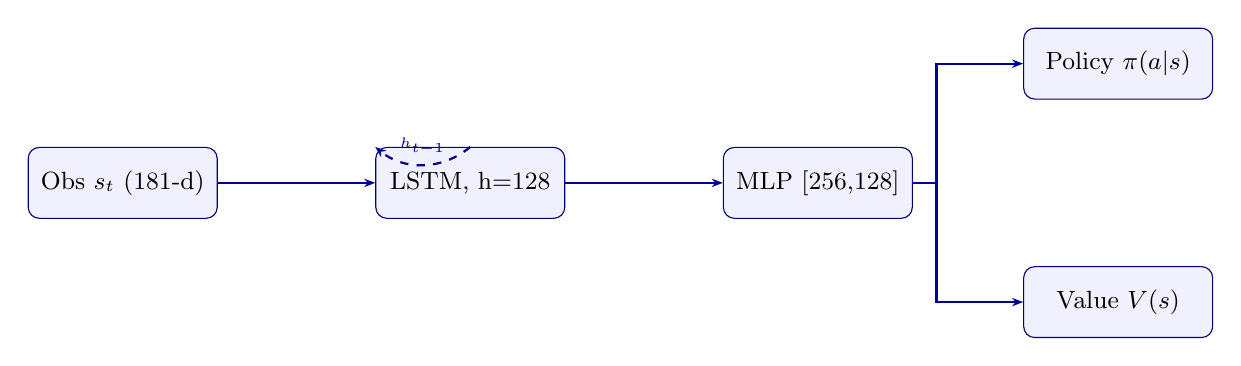
\begin{tikzpicture}[node distance=1.5cm,
  box/.style={rectangle,rounded corners=4pt,draw=blue!50!black,
              fill=blue!6,minimum width=2.4cm,minimum height=0.9cm,font=\small},
  arr/.style={-{Stealth[length=4pt]},thick,blue!60!black}]
  \node[box] (obs)  {Obs $s_t$ (181-d)};
  \node[box,right=2cm of obs]  (lstm) {LSTM, h=128};
  \node[box,right=2cm of lstm] (mlp)  {MLP [256,128]};
  \node[box,above right=0.6cm and 1.4cm of mlp] (pol) {Policy $\pi(a|s)$};
  \node[box,below right=0.6cm and 1.4cm of mlp] (val) {Value $V(s)$};
  \draw[arr] (obs)--(lstm);
  \draw[arr] (lstm)--(mlp);
  \draw[arr] (mlp.east)--++(0.3,0)|-(pol.west);
  \draw[arr] (mlp.east)--++(0.3,0)|-(val.west);
  \draw[arr,dashed] (lstm.north) to[bend left=40]
        node[above,font=\tiny]{$h_{t-1}$} (lstm.north west);
\end{tikzpicture}
\caption{RecurrentPPO architecture. The LSTM processes observations
sequentially, maintaining hidden state $h_t$ across time steps.
Separate MLP heads decode policy logits and state value.}
\label{fig:arch}
\end{figure}

The LSTM is the key architectural improvement over a flat MLP. It captures
sequential dependencies that matter for finance: momentum persistence,
volatility clustering, and regime transitions that unfold over multiple days.
A flat MLP treating the 20-day window as an unordered vector cannot represent
these patterns.

\begin{table}[H]
\centering
\caption{RecurrentPPO hyperparameters.}
\label{tab:hparams}
\begin{tabular}{ll|ll}
\toprule
\textbf{Parameter} & \textbf{Value} & \textbf{Parameter} & \textbf{Value} \\
\midrule
LSTM hidden   & 128     & Learning rate        & $10^{-4}$ \\
LSTM layers   & 1       & Clip range           & 0.15 \\
MLP           & [256,128]& Entropy coeff.      & 0.05 \\
Training steps& 300k    & GAE $\lambda$        & 0.95 \\
Batch size    & 128     & Discount $\gamma$    & 0.995 \\
\bottomrule
\end{tabular}
\end{table}

\section{Equity Results}

\subsection{Price Overview}

\begin{figure}[H]
  \centering
  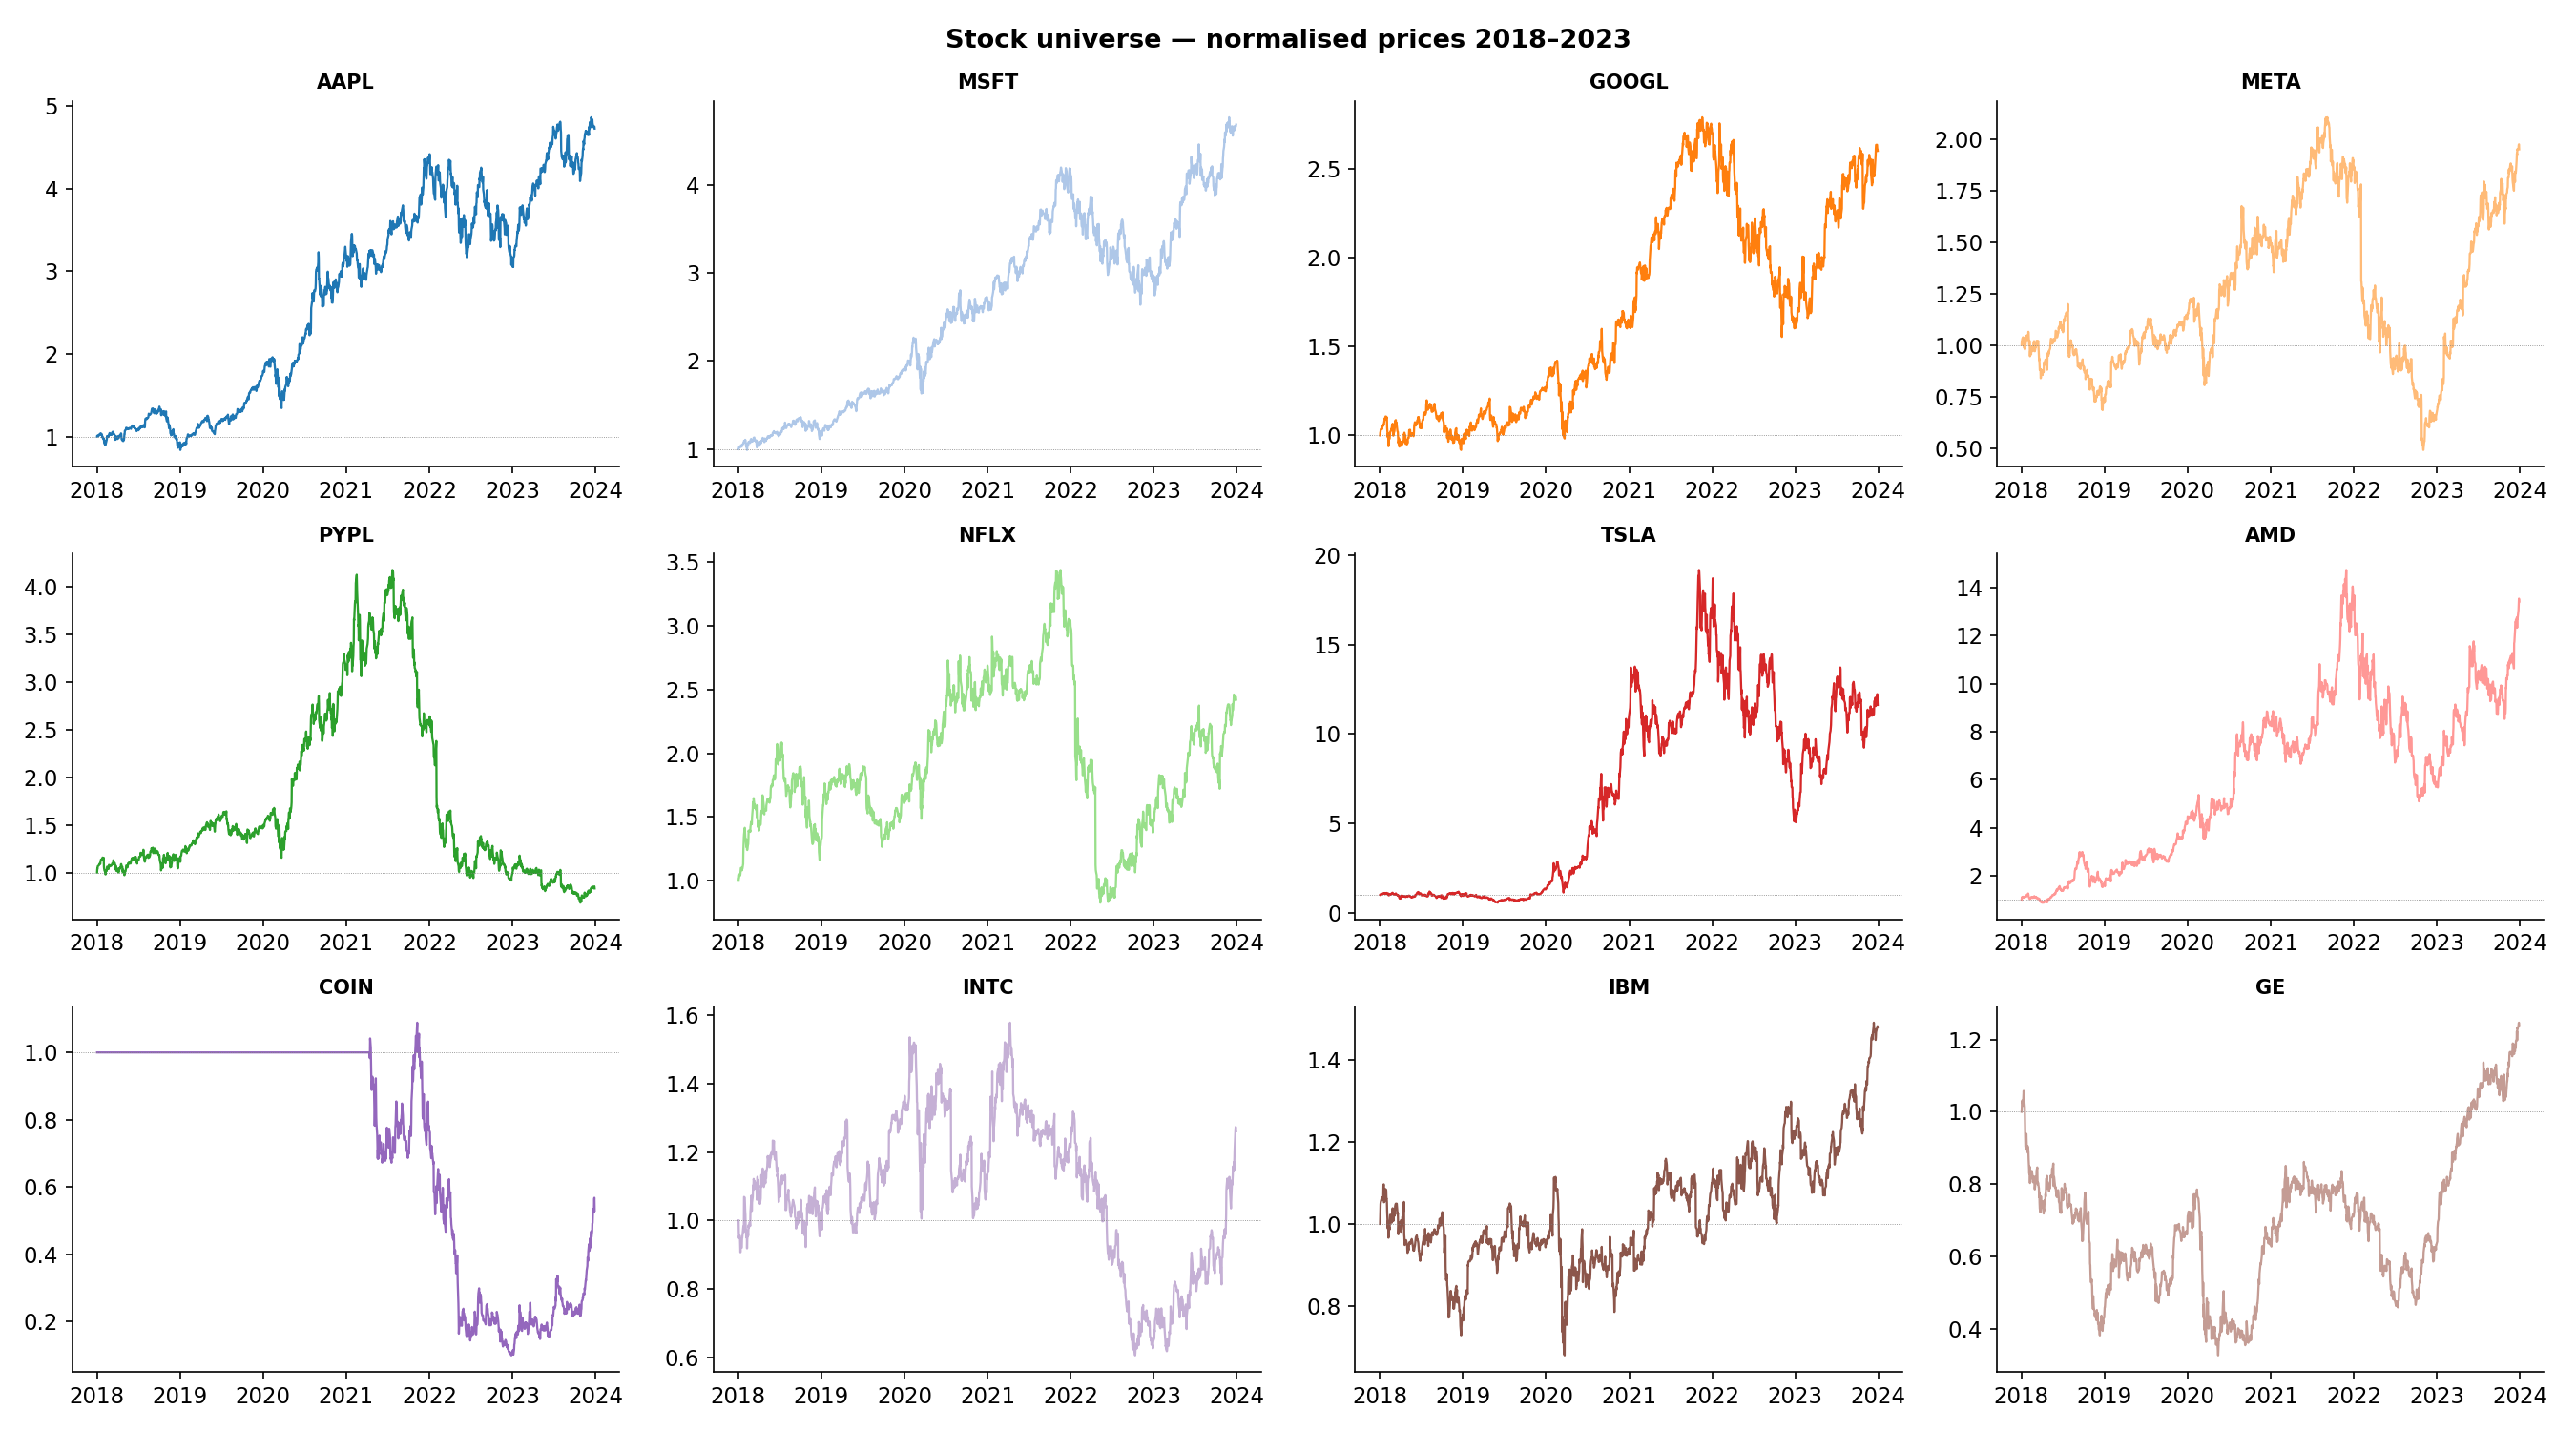
\includegraphics[width=\textwidth]{figures/stock_price_overview.png}
  \caption{Full price history of the equity universe (normalised, 2018--2023).
  Blue shading: Period~A training. Red shading: Period~A test. The 2022
  tech selloff is clearly visible across the portfolio.}
  \label{fig:stock_prices}
\end{figure}

\subsection{Period A: Bull Train, Bear+Recovery Test}

Period~A trains on 2018--2021 (bullish with COVID recovery) and tests on
2022--2023 (tech selloff then partial recovery). It tests whether a
bull-trained agent handles a genuine regime shift. Complete numerical
results for all 12 equities are in Table~\ref{tab:equity_results}; figures
below show four representative assets illustrating the main phenomena.

\begin{figure}[H]
  \centering
  \begin{subfigure}[b]{0.49\textwidth}
    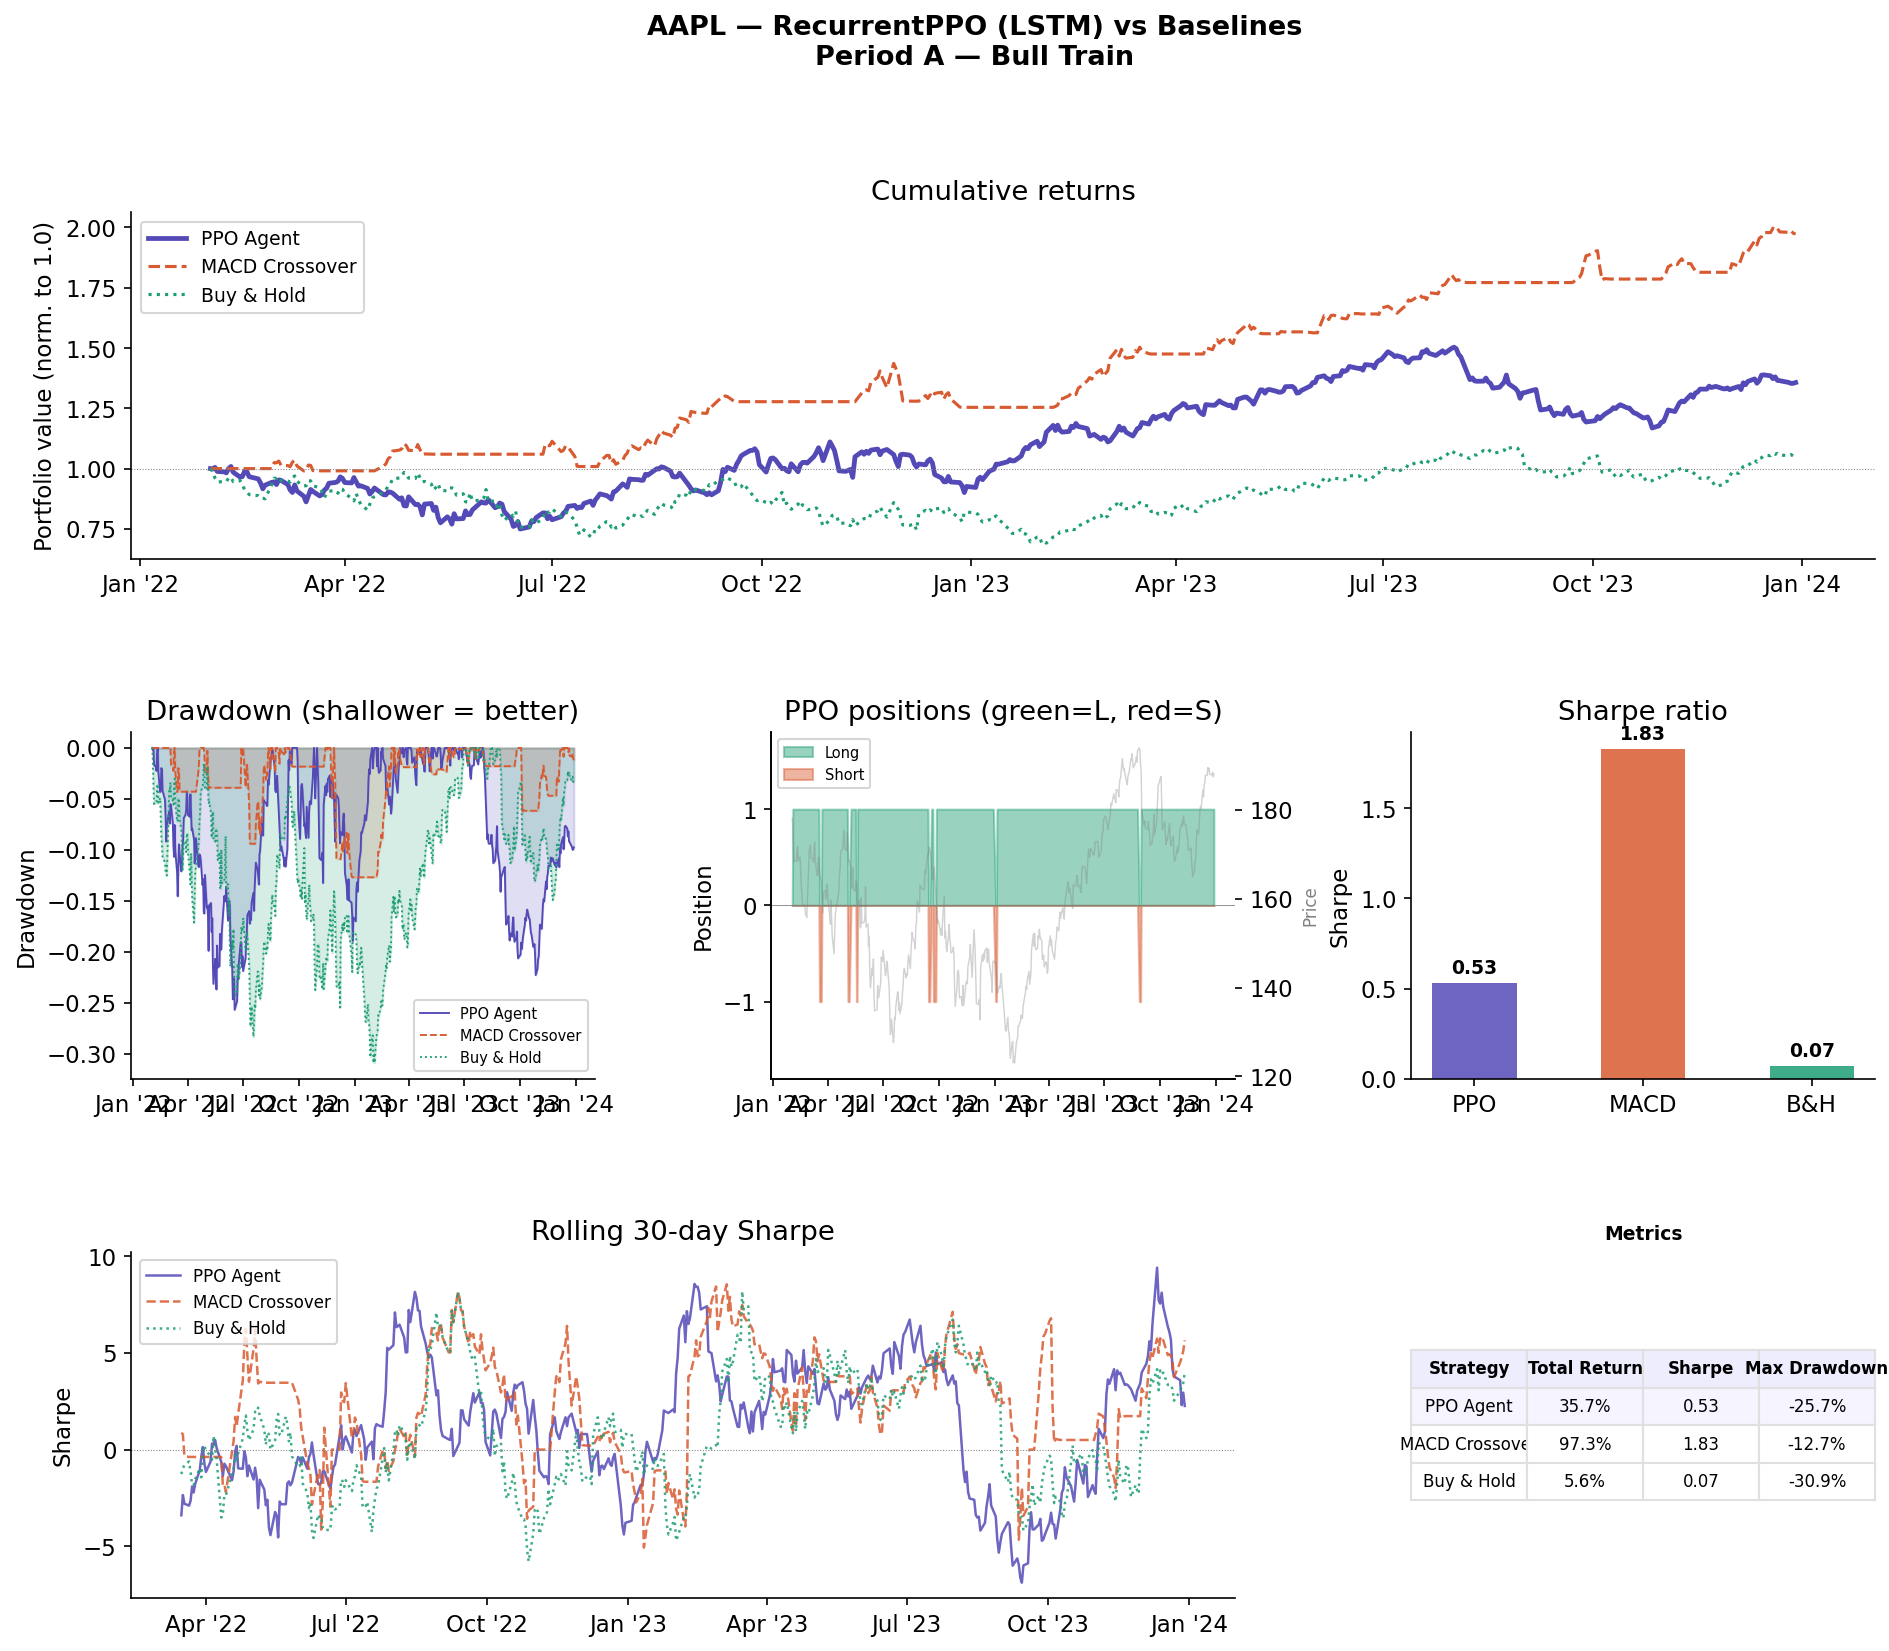
\includegraphics[width=\textwidth]{figures/stocks_a/AAPL.png}
    \caption{AAPL --- Period A}
  \end{subfigure}\hfill
  \begin{subfigure}[b]{0.49\textwidth}
    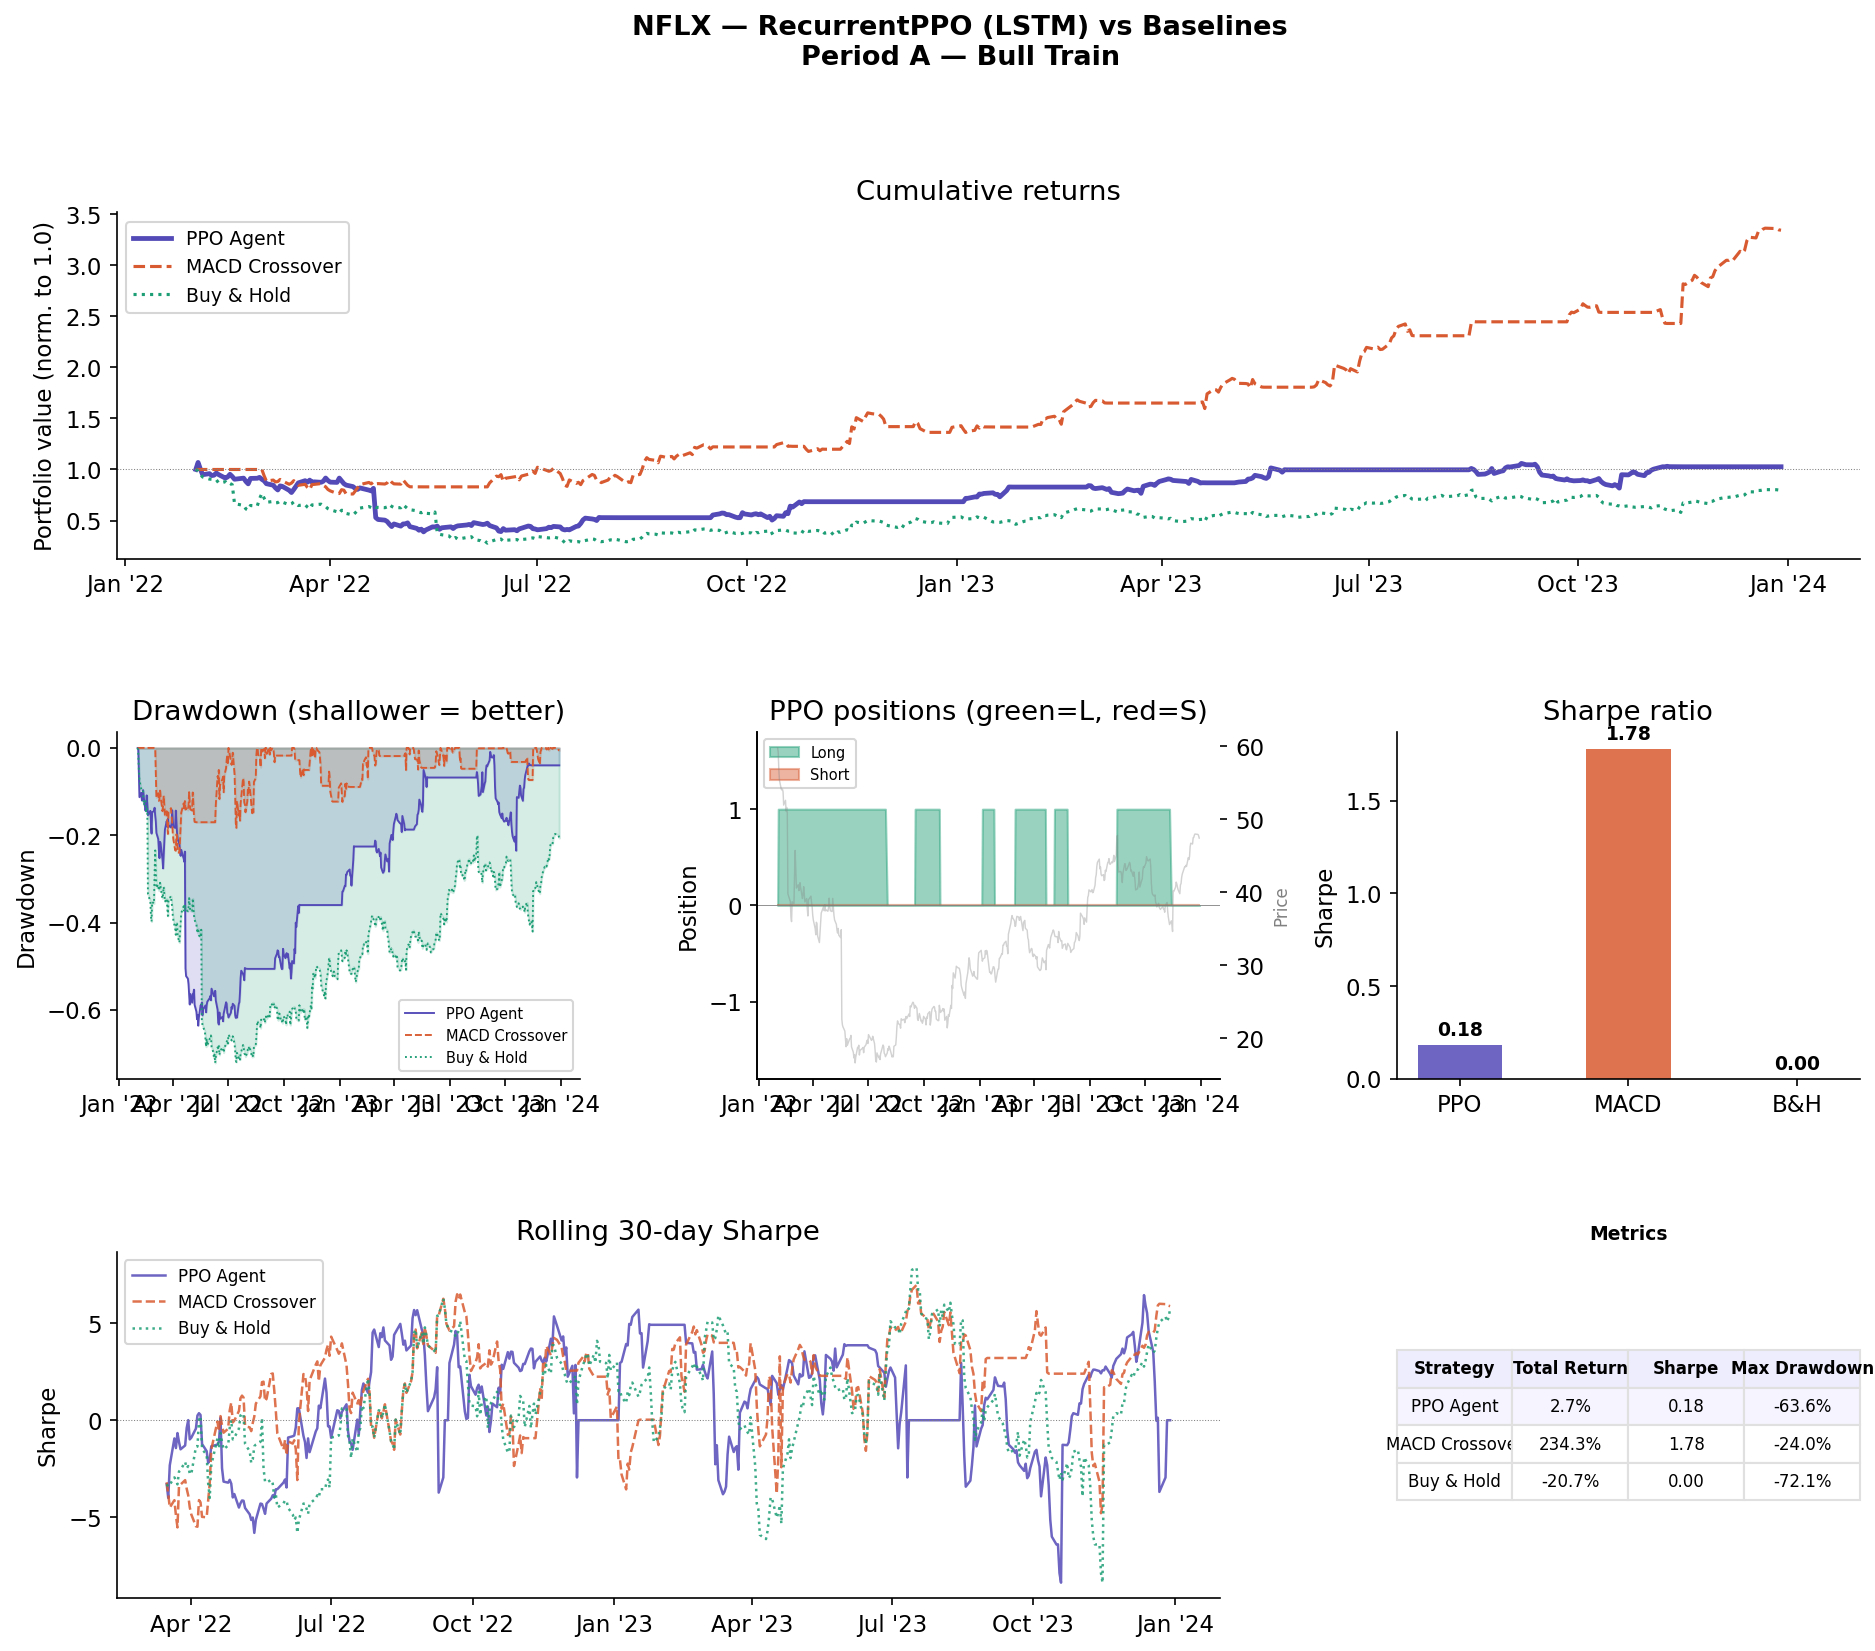
\includegraphics[width=\textwidth]{figures/stocks_a/NFLX.png}
    \caption{NFLX --- Period A}
  \end{subfigure}
  \caption{AAPL (bull stock): PPO $+35.7$\% (Sharpe~0.53) vs B\&H $+5.6$\%
  (Sharpe~0.07)---contrary to expectation, the agent outperforms the passive
  strategy on both return and Sharpe in Period~A, suggesting the LSTM
  captured meaningful timing signals even on a bull stock.
  NFLX (crash stock): PPO $+2.7$\% (Sharpe~0.18) vs B\&H $-20.7$\%
  (Sharpe~0.00)---short positioning delivers a positive return while
  B\&H absorbs the full 2022 loss.}
  \label{fig:stocks_a_aapl_nflx}
\end{figure}

\begin{figure}[H]
  \centering
  \begin{subfigure}[b]{0.49\textwidth}
    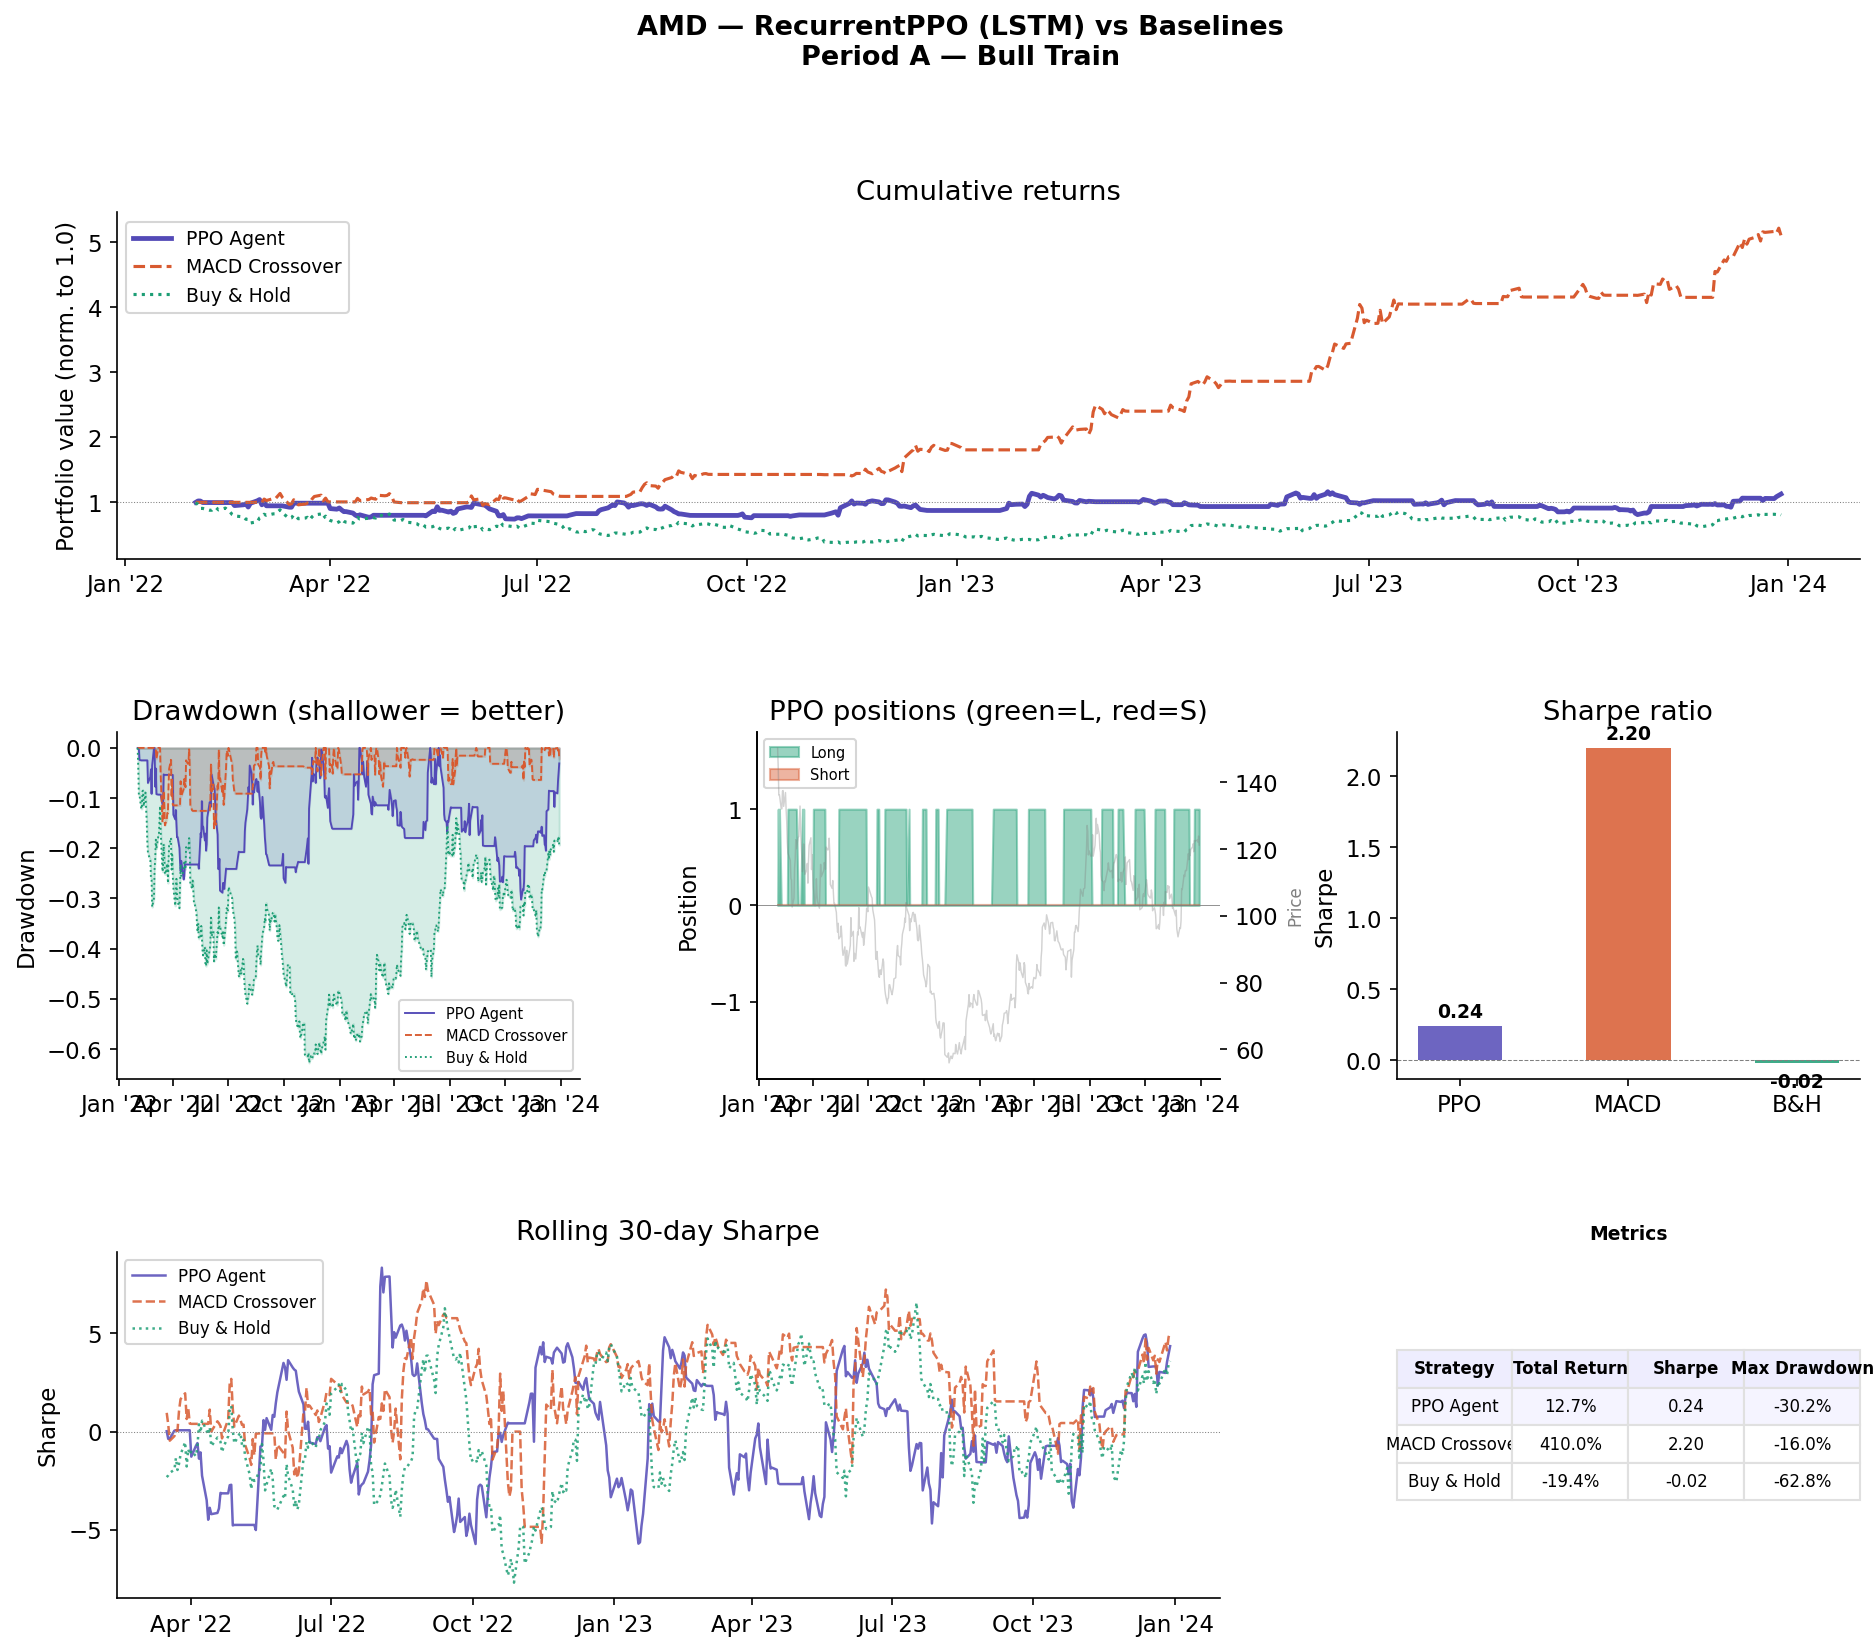
\includegraphics[width=\textwidth]{figures/stocks_a/AMD.png}
    \caption{AMD --- Period A}
  \end{subfigure}\hfill
  \begin{subfigure}[b]{0.49\textwidth}
    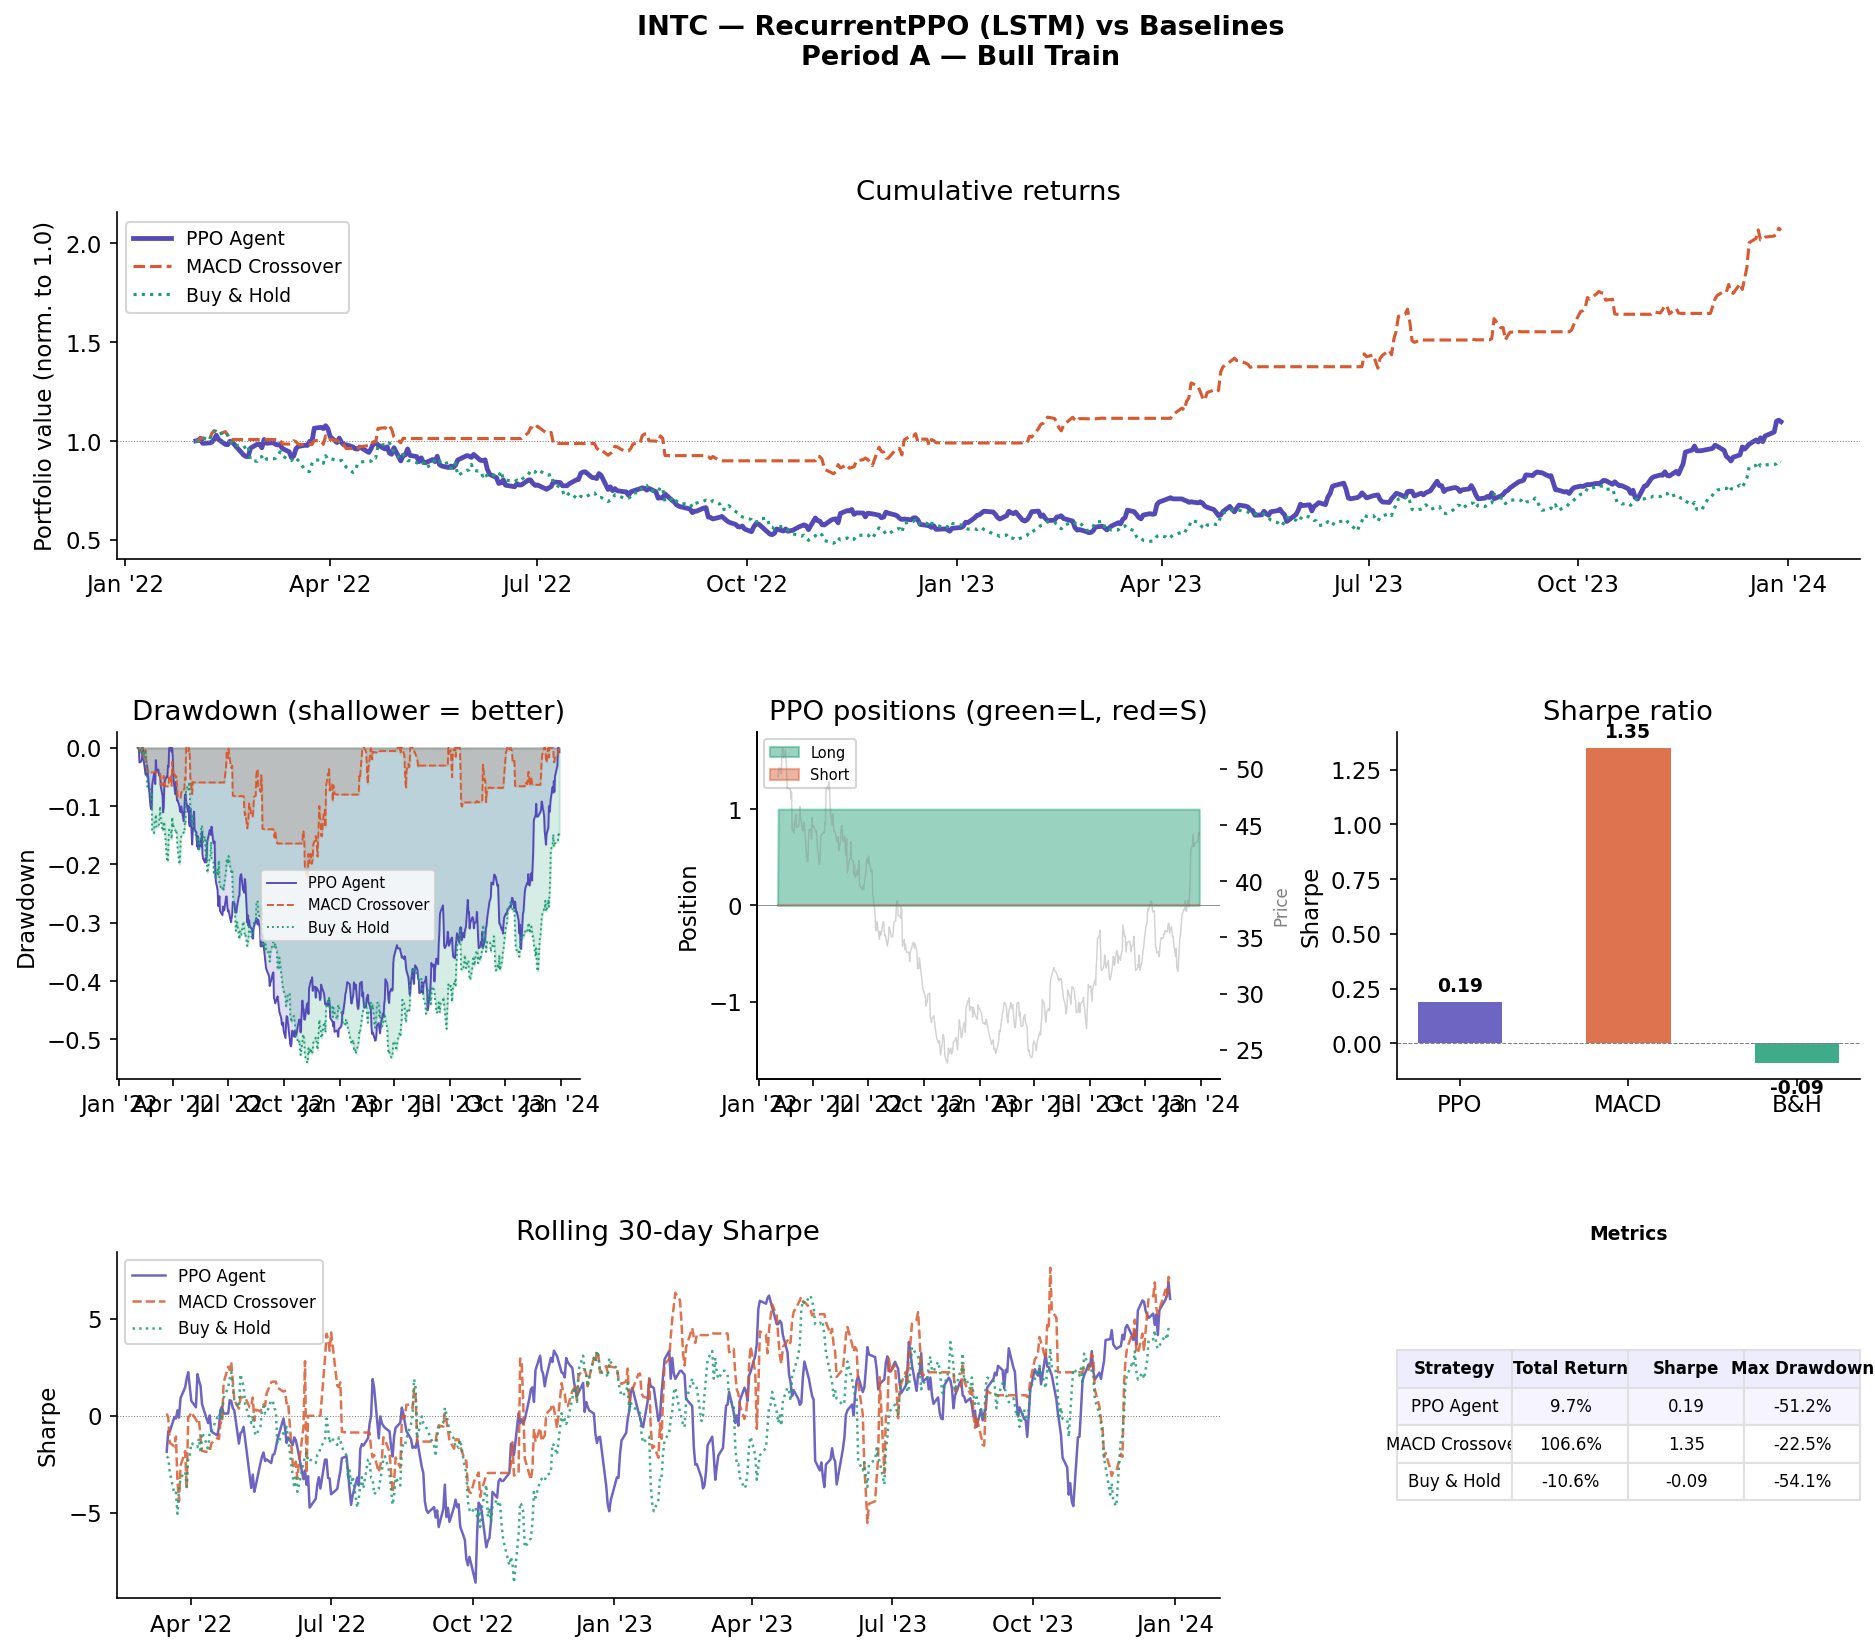
\includegraphics[width=\textwidth]{figures/stocks_a/INTC.png}
    \caption{INTC --- Period A}
  \end{subfigure}
 \caption{AMD (volatile): PPO $+12.7$\% (Sharpe~0.24) vs B\&H $-19.4$\%
  (Sharpe~$-0.02$)---the agent avoids the 2022 AMD selloff and outperforms
  on both return and risk-adjusted metrics, despite MACD dominating on the
  strong 2021 rally (+296.8\%). INTC (sideways): PPO $+9.7$\% (Sharpe~0.19)
  vs B\&H $-10.6$\% (Sharpe~$-0.09$)---PPO beats B\&H on both metrics in
  a low-signal range-bound stock, preserving capital while the passive
  strategy loses ground.}
  \label{fig:stocks_a_amd_intc}
\end{figure}

\subsection{Period B: Mixed Train, Bear-to-Recovery Test}

Period~B trains on 2019--June~2022 (including the full 2022 bear market)
and tests on July~2022--2023. The agent has now experienced bear conditions
during training. Complete results in Table~\ref{tab:equity_results};
figures show the two most instructive assets.

\begin{figure}[H]
  \centering
  \begin{subfigure}[b]{0.49\textwidth}
    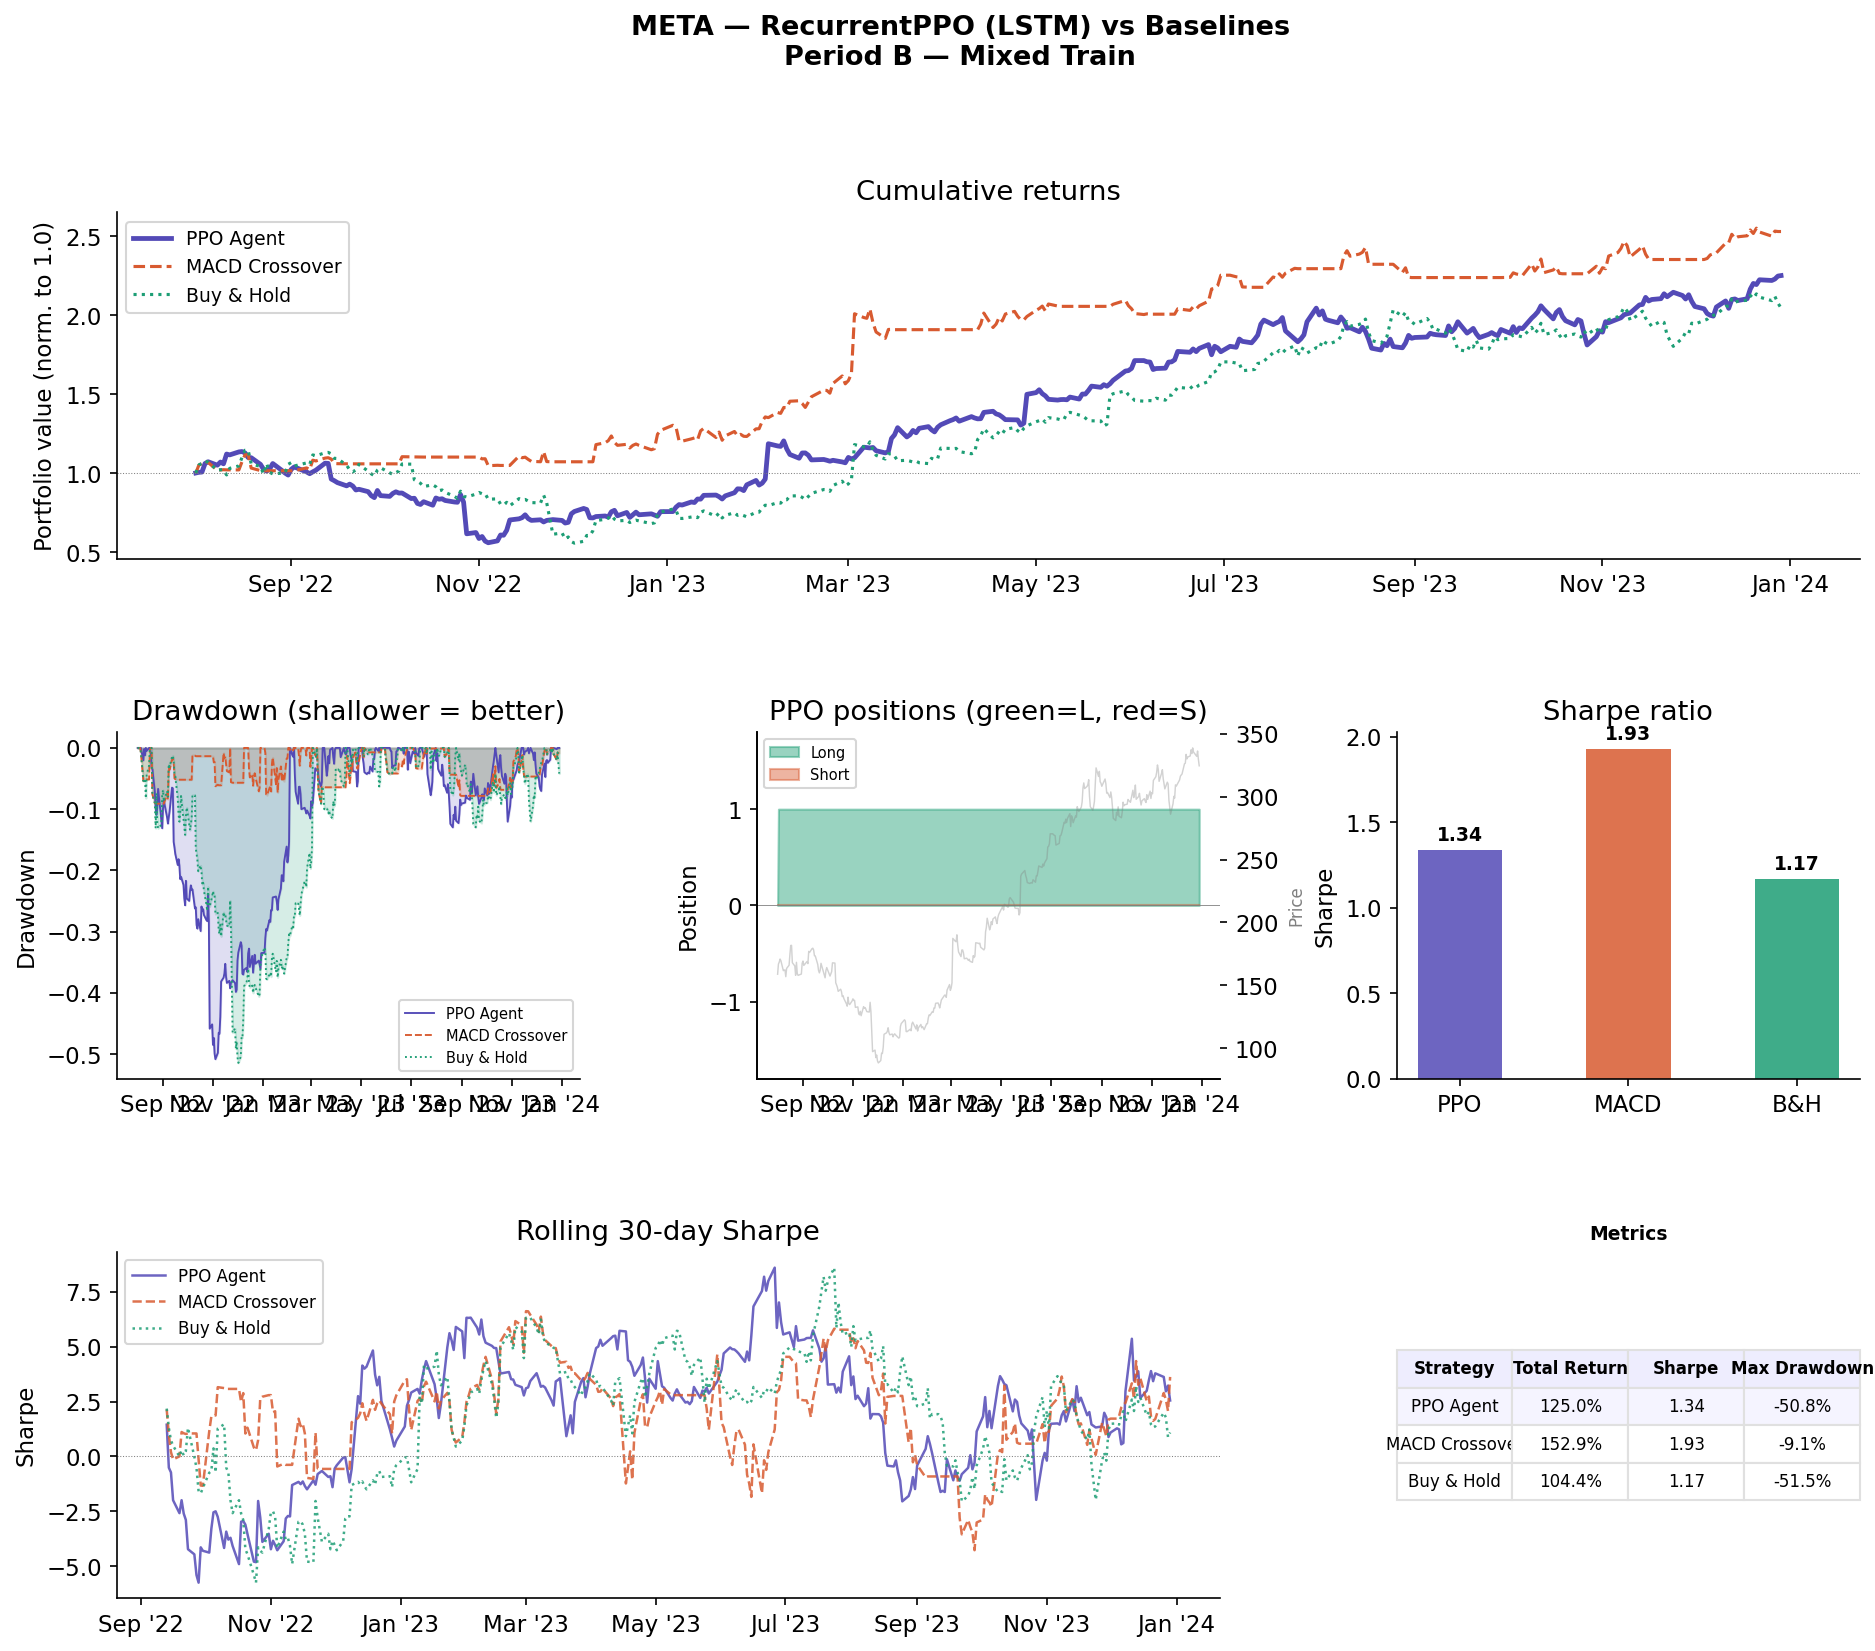
\includegraphics[width=\textwidth]{figures/stocks_b/META.png}
    \caption{META --- Period B}
  \end{subfigure}\hfill
  \begin{subfigure}[b]{0.49\textwidth}
    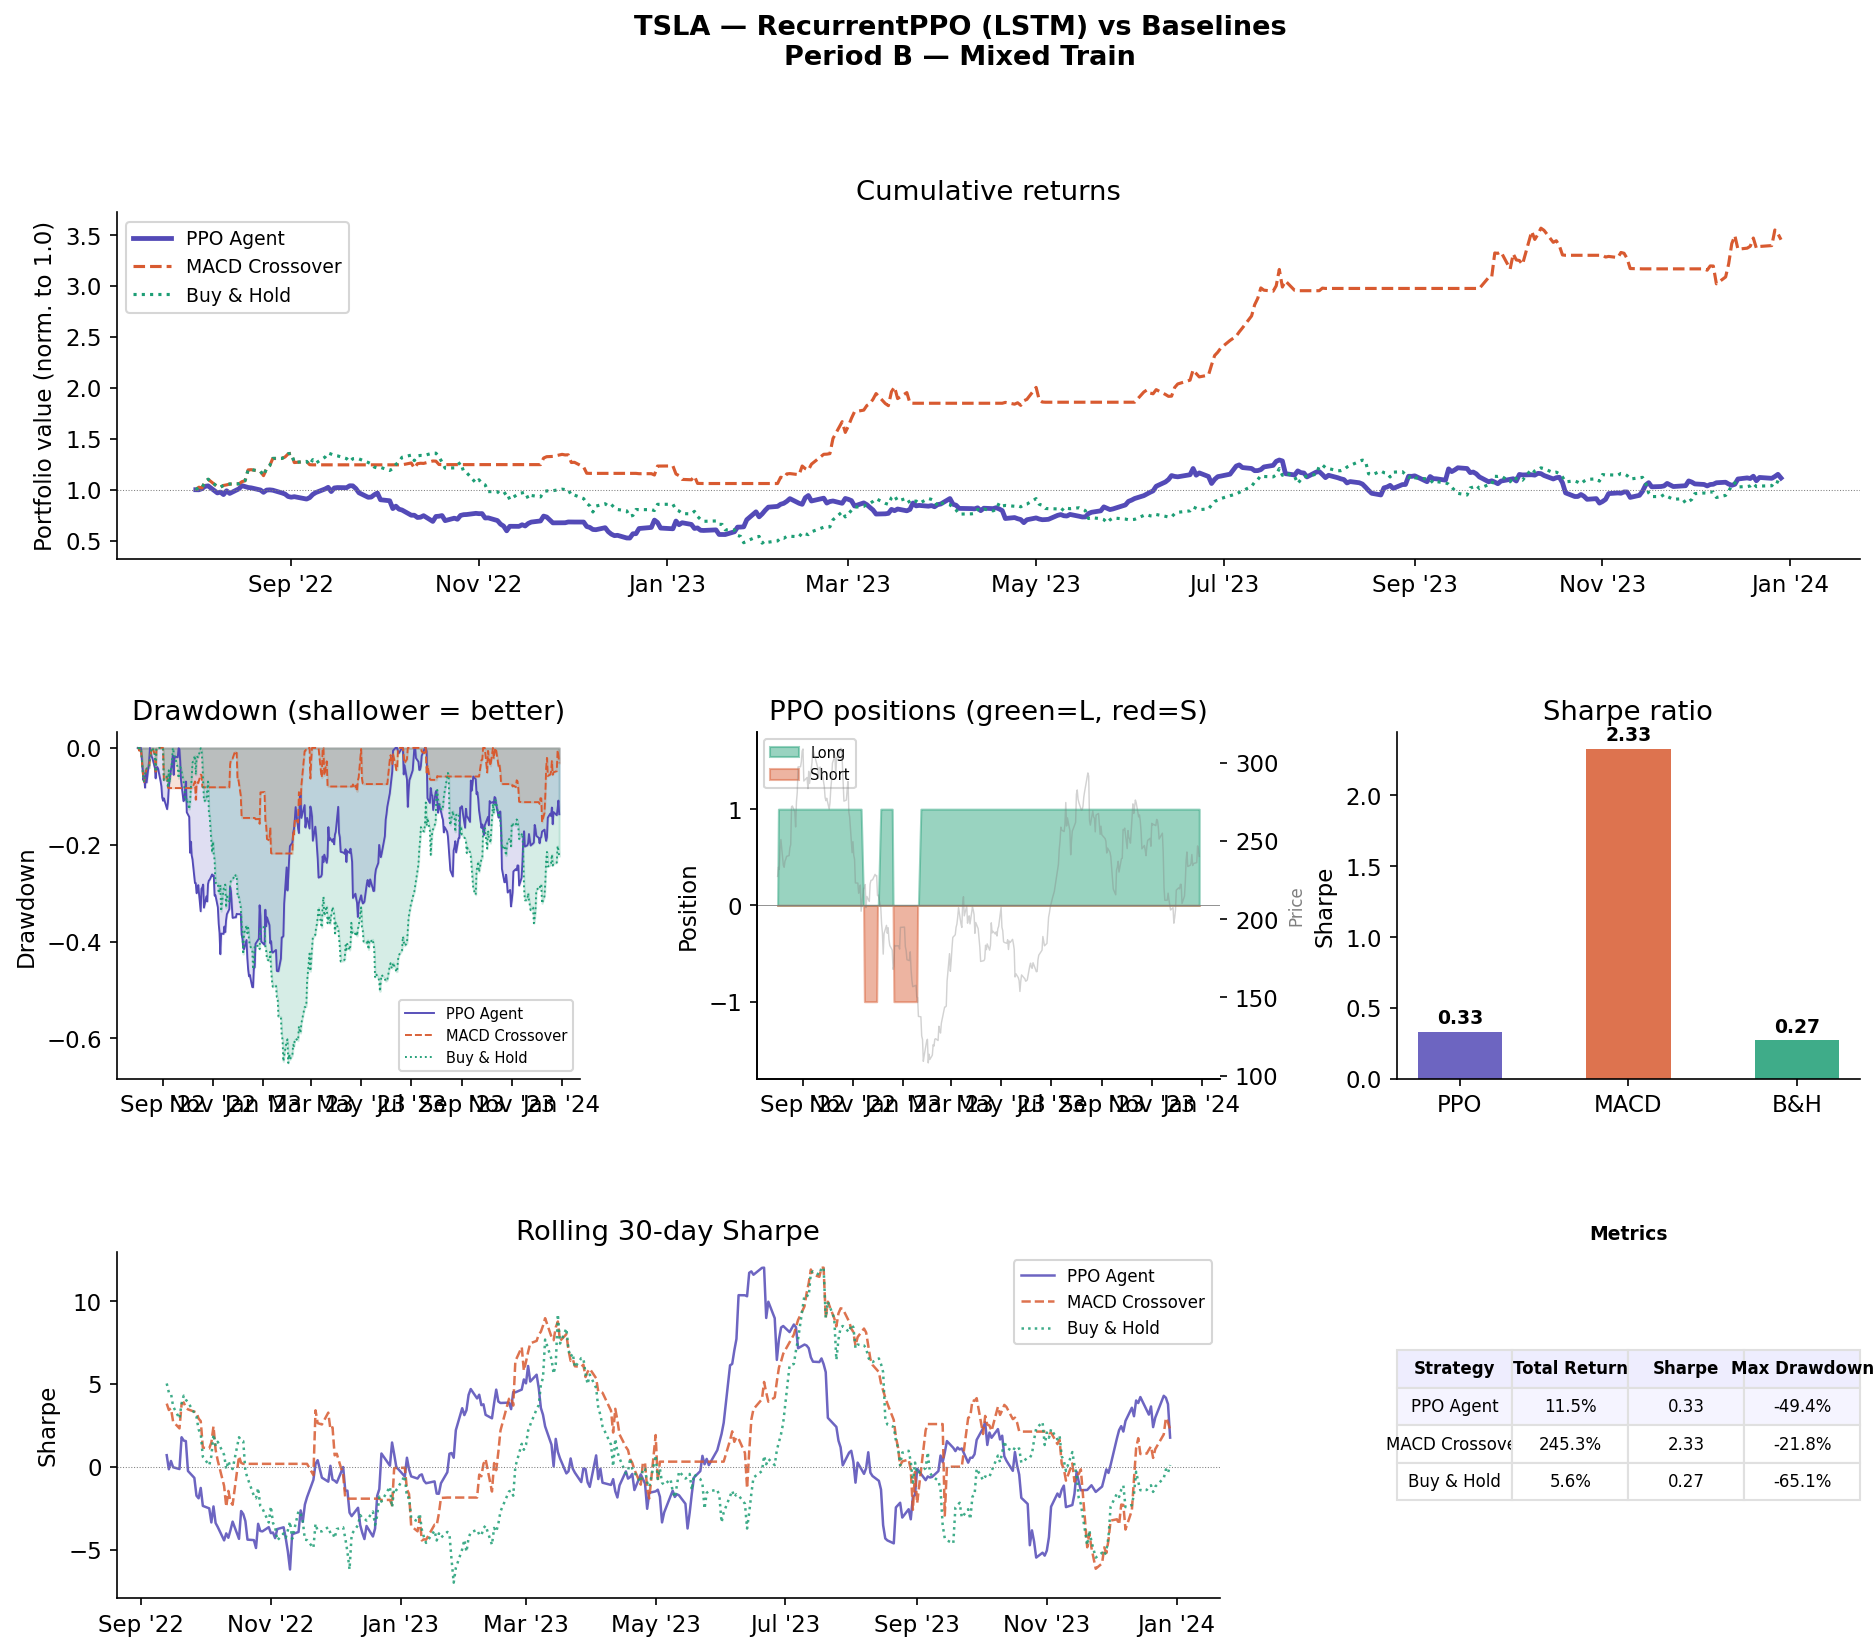
\includegraphics[width=\textwidth]{figures/stocks_b/TSLA.png}
    \caption{TSLA --- Period B}
  \end{subfigure}
  \caption{META Period~B: PPO $+125.0$\% (Sharpe~1.34) vs B\&H $+104.4$\%
  (Sharpe~1.17)---the clearest case of genuine total return outperformance
  enabled by mixed training. TSLA Period~B: PPO $+11.5$\% (Sharpe~0.33)
  vs B\&H $+5.6$\% (Sharpe~0.27)---mixed training produces a positive,
  outperforming policy on TSLA; the agent beats B\&H on both return and
  Sharpe, a marked contrast to the degenerate flat policy seen in Period~A.}
  \label{fig:stocks_b_meta_tsla}
\end{figure}

\subsection{Equity Results}

\begin{tabular}{llrrrrrr}
\toprule
& & \multicolumn{3}{c}{\textbf{Period A} (Test 2022--2023)} &
  \multicolumn{3}{c}{\textbf{Period B} (Test 2022H2--2023)} \\
\cmidrule(lr){3-5}\cmidrule(lr){6-8}
\textbf{Asset} & \textbf{Strategy} &
  \textbf{Return} & \textbf{Sharpe} & \textbf{Max DD} &
  \textbf{Return} & \textbf{Sharpe} & \textbf{Max DD} \\
\midrule
\multirow{3}{*}{AAPL}
  & PPO   & \cellcolor{wingreen}$35.7\%$ & \cellcolor{wingreen}$0.53$ & \cellcolor{wingreen}$-25.7\%$ & $20.0\%$ & $0.43$ & $-28.3\%$ \\
  & MACD  & $97.3\%$ & $1.83$ & $-12.7\%$ & $90.6\%$ & $2.42$ & $-12.7\%$ \\
  & B\&H  & $5.6\%$ & $0.07$ & $-30.9\%$ & $37.9\%$ & $0.79$ & $-28.3\%$ \\
\midrule
\multirow{3}{*}{MSFT}
  & PPO   & \cellcolor{wingreen}$22.8\%$ & \cellcolor{wingreen}$0.34$ & \cellcolor{wingreen}$-31.8\%$ & $35.4\%$ & $0.72$ & $-26.8\%$ \\
  & MACD  & $89.8\%$ & $1.38$ & $-9.6\%$ & $95.4\%$ & $1.97$ & $-9.5\%$ \\
  & B\&H  & $15.3\%$ & $0.23$ & $-35.6\%$ & $48.0\%$ & $0.92$ & $-26.8\%$ \\
\midrule
\multirow{3}{*}{GOOGL}
  & PPO   & \cellcolor{wingreen}$3.5\%$ & \cellcolor{wingreen}$0.08$ & \cellcolor{wingreen}$-43.6\%$ & $20.4\%$ & $0.41$ & $-31.7\%$ \\
  & MACD  & $62.7\%$ & $0.97$ & $-12.0\%$ & $65.6\%$ & $1.41$ & $-10.8\%$ \\
  & B\&H  & $-8.6\%$ & $-0.10$ & $-43.6\%$ & $21.9\%$ & $0.43$ & $-31.7\%$ \\
\midrule
\multirow{3}{*}{META}
  & PPO   & $-19.6\%$ & $-0.05$ & $-77.6\%$ & \cellcolor{wingreen}$125.0\%$ & \cellcolor{wingreen}$1.34$ & \cellcolor{wingreen}$-50.8\%$ \\
  & MACD  & $127.2\%$ & $1.26$ & $-18.8\%$ & $152.9\%$ & $1.93$ & $-9.1\%$ \\
  & B\&H  & $-3.4\%$ & $0.16$ & $-73.7\%$ & $104.4\%$ & $1.17$ & $-51.5\%$ \\
\midrule
\multirow{3}{*}{PYPL}
  & PPO   & \cellcolor{wingreen}$-64.3\%$ & \cellcolor{wingreen}$-0.96$ & \cellcolor{wingreen}$-72.1\%$ & $-30.3\%$ & $-0.60$ & $-52.8\%$ \\
  & MACD  & $125.8\%$ & $1.35$ & $-17.1\%$ & $113.1\%$ & $1.83$ & $-11.5\%$ \\
  & B\&H  & $-70.4\%$ & $-1.14$ & $-74.2\%$ & $-19.3\%$ & $-0.27$ & $-50.6\%$ \\
\midrule
\multirow{3}{*}{NFLX}
  & PPO   & \cellcolor{wingreen}$2.7\%$ & \cellcolor{wingreen}$0.18$ & \cellcolor{wingreen}$-63.6\%$ & $117.9\%$ & $1.36$ & $-27.5\%$ \\
  & MACD  & $234.3\%$ & $1.78$ & $-24.0\%$ & $242.9\%$ & $2.65$ & $-12.4\%$ \\
  & B\&H  & $-20.7\%$ & $0.00$ & $-72.1\%$ & $163.4\%$ & $1.62$ & $-27.5\%$ \\
\midrule
\multirow{3}{*}{TSLA}
  & PPO   & \cellcolor{wingreen}$-19.0\%$ & \cellcolor{wingreen}$0.03$ & \cellcolor{wingreen}$-71.7\%$ & \cellcolor{wingreen}$11.5\%$ & \cellcolor{wingreen}$0.33$ & \cellcolor{wingreen}$-49.4\%$ \\
  & MACD  & $319.0\%$ & $1.92$ & $-21.2\%$ & $245.3\%$ & $2.33$ & $-21.8\%$ \\
  & B\&H  & $-40.0\%$ & $-0.21$ & $-73.0\%$ & $5.6\%$ & $0.27$ & $-65.1\%$ \\
\midrule
\multirow{3}{*}{AMD}
  & PPO   & \cellcolor{wingreen}$12.7\%$ & \cellcolor{wingreen}$0.24$ & \cellcolor{wingreen}$-30.2\%$ & $-11.2\%$ & $-1.35$ & $-15.9\%$ \\
  & MACD  & $410.0\%$ & $2.20$ & $-16.0\%$ & $379.0\%$ & $3.04$ & $-8.1\%$ \\
  & B\&H  & $-19.4\%$ & $-0.02$ & $-62.8\%$ & $64.5\%$ & $0.85$ & $-46.2\%$ \\
\midrule
\multirow{3}{*}{COIN}
  & PPO   & \cellcolor{wingreen}$-2.1\%$ & \cellcolor{wingreen}$0.44$ & \cellcolor{wingreen}$-84.8\%$ & $-90.2\%$ & $-1.33$ & $-92.4\%$ \\
  & MACD  & $392.2\%$ & $1.40$ & $-44.2\%$ & $407.7\%$ & $1.78$ & $-40.1\%$ \\
  & B\&H  & $-50.3\%$ & $0.08$ & $-87.0\%$ & $154.3\%$ & $1.10$ & $-66.8\%$ \\
\midrule
\multirow{3}{*}{IBM}
  & PPO   & $-5.4\%$ & $-0.39$ & $-20.3\%$ & \cellcolor{wingreen}$34.5\%$ & \cellcolor{wingreen}$0.97$ & \cellcolor{wingreen}$-17.6\%$ \\
  & MACD  & $91.6\%$ & $2.20$ & $-8.0\%$ & $65.4\%$ & $2.55$ & $-8.0\%$ \\
  & B\&H  & $28.4\%$ & $0.50$ & $-17.6\%$ & $20.8\%$ & $0.54$ & $-17.6\%$ \\
\midrule
\multirow{3}{*}{INTC}
  & PPO   & \cellcolor{wingreen}$9.7\%$ & \cellcolor{wingreen}$0.19$ & \cellcolor{wingreen}$-51.2\%$ & $-15.6\%$ & $-0.36$ & $-40.1\%$ \\
  & MACD  & $106.6\%$ & $1.35$ & $-22.5\%$ & $150.5\%$ & $2.31$ & $-10.1\%$ \\
  & B\&H  & $-10.6\%$ & $-0.09$ & $-54.1\%$ & $28.9\%$ & $0.52$ & $-37.7\%$ \\
\midrule
\multirow{3}{*}{GE}
  & PPO   & \cellcolor{wingreen}$53.1\%$ & \cellcolor{wingreen}$0.74$ & \cellcolor{wingreen}$-49.0\%$ & $14.0\%$ & $0.45$ & $-5.2\%$ \\
  & MACD  & $184.4\%$ & $2.55$ & $-12.5\%$ & $193.8\%$ & $3.61$ & $-5.7\%$ \\
  & B\&H  & $63.2\%$ & $0.83$ & $-40.7\%$ & $146.7\%$ & $2.29$ & $-23.5\%$ \\
\bottomrule
\end{tabular}

\section{Cryptocurrency Results}

Crypto uses a single mixed-regime training period (2019--2022H1, including
the crash) tested on 2022H2--2023. Full results for all 5 assets are in
Table~\ref{tab:crypto_results}; the two figures below show BNB and SOL as
the most instructive representatives.

\begin{figure}[H]
  \centering
  \begin{subfigure}[b]{0.49\textwidth}
    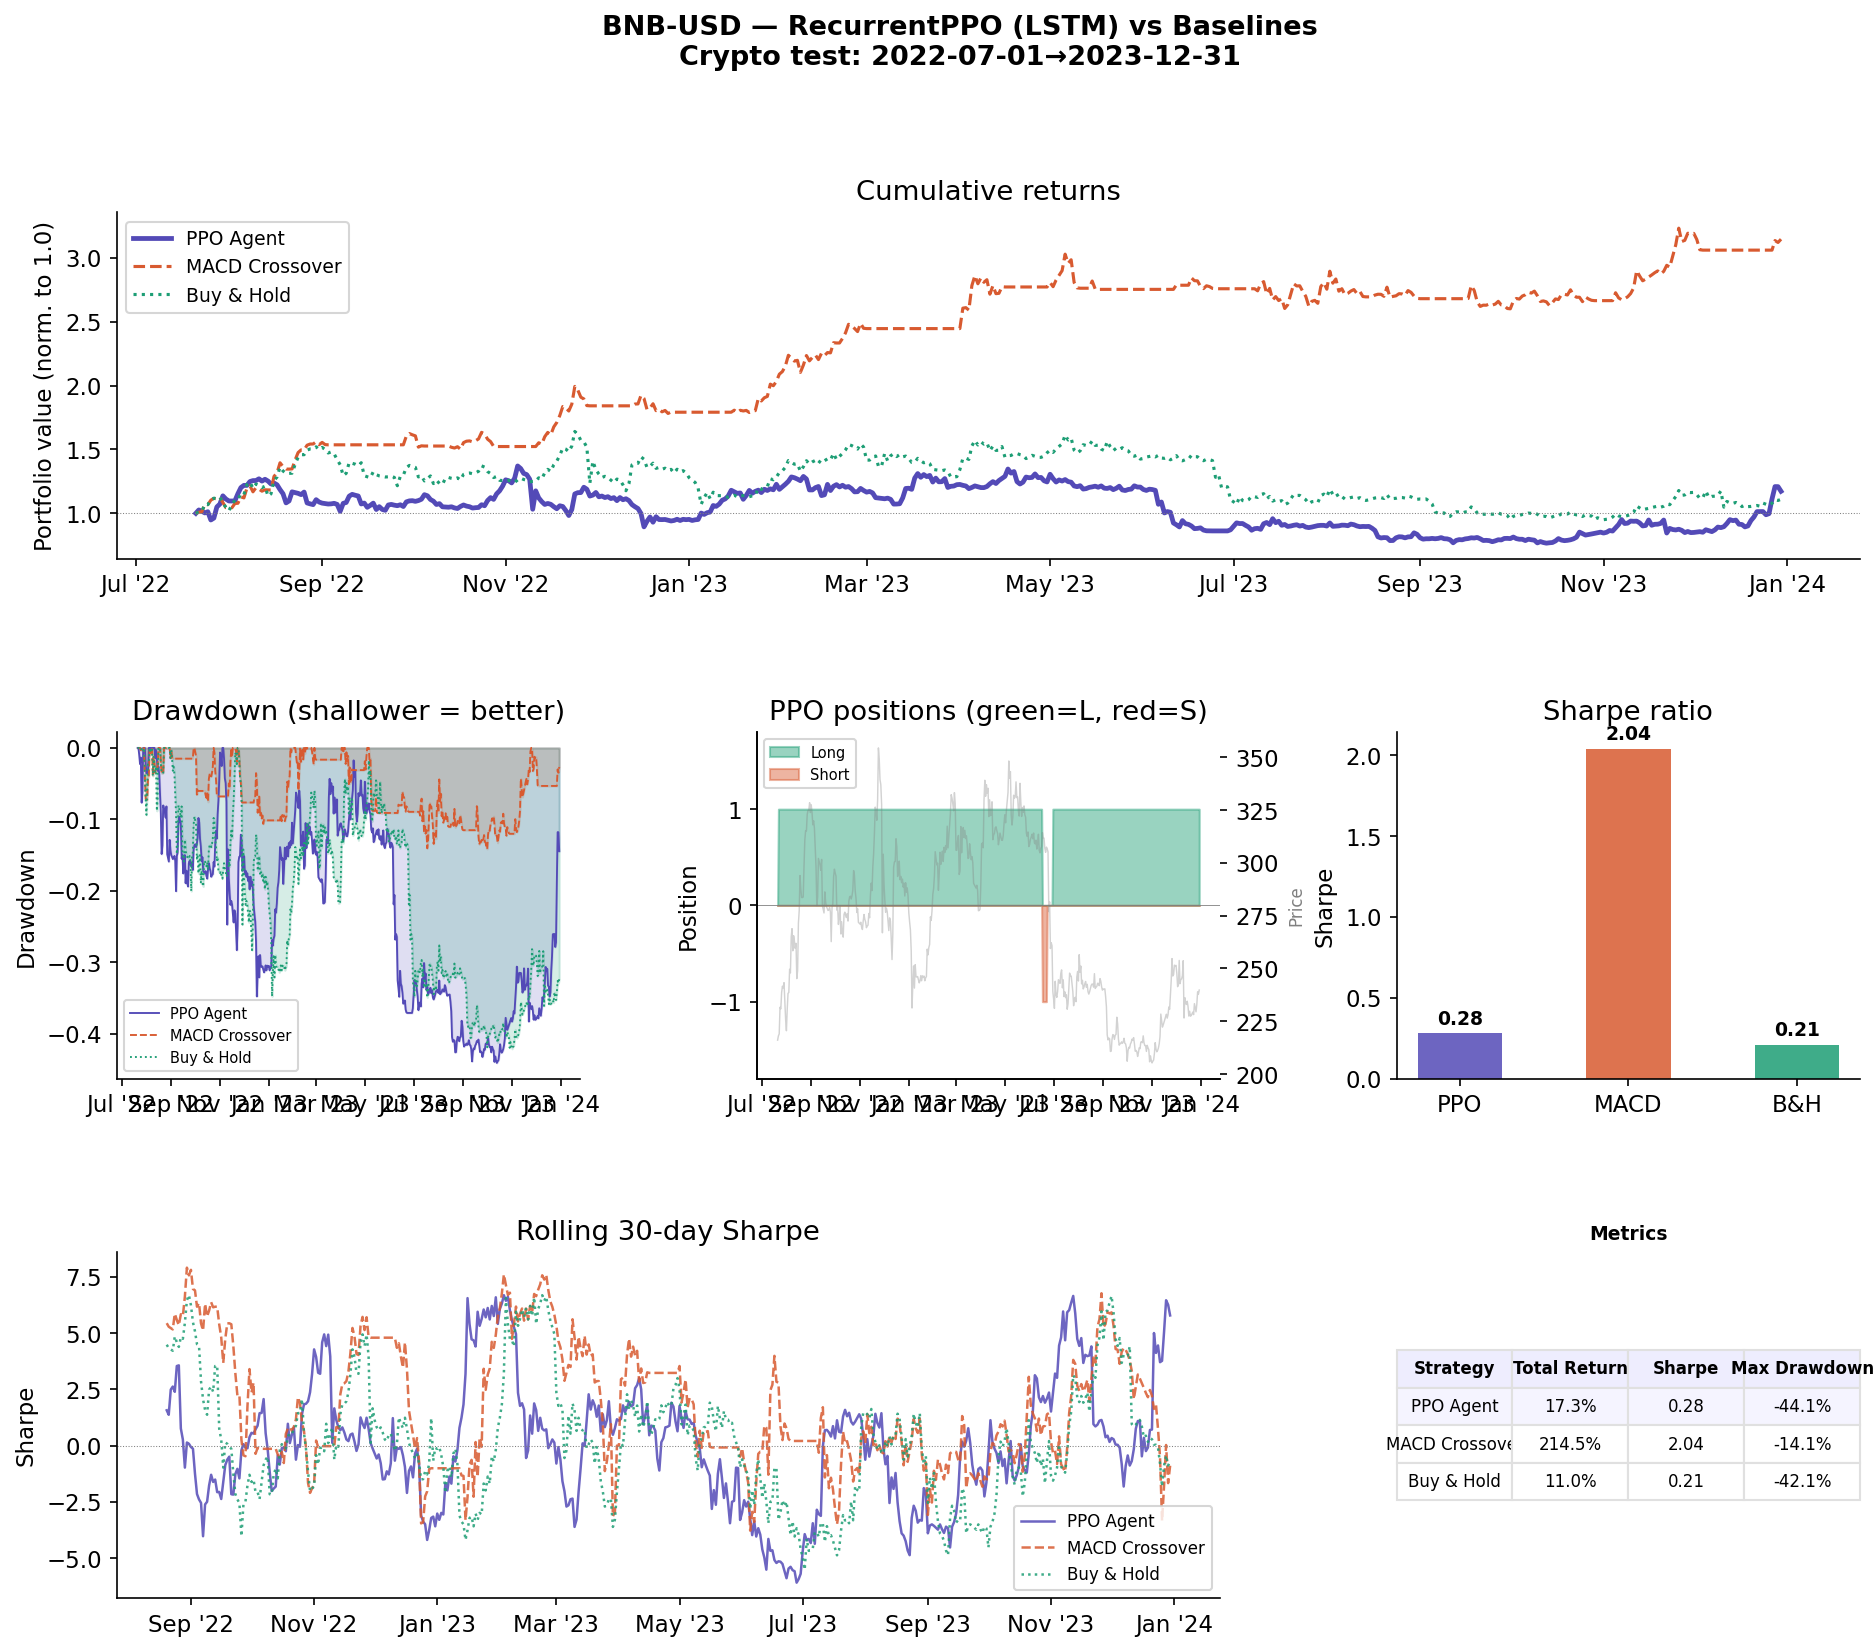
\includegraphics[width=\textwidth]{figures/crypto/BNB.png}
    \caption{BNB-USD}
  \end{subfigure}\hfill
  \begin{subfigure}[b]{0.49\textwidth}
    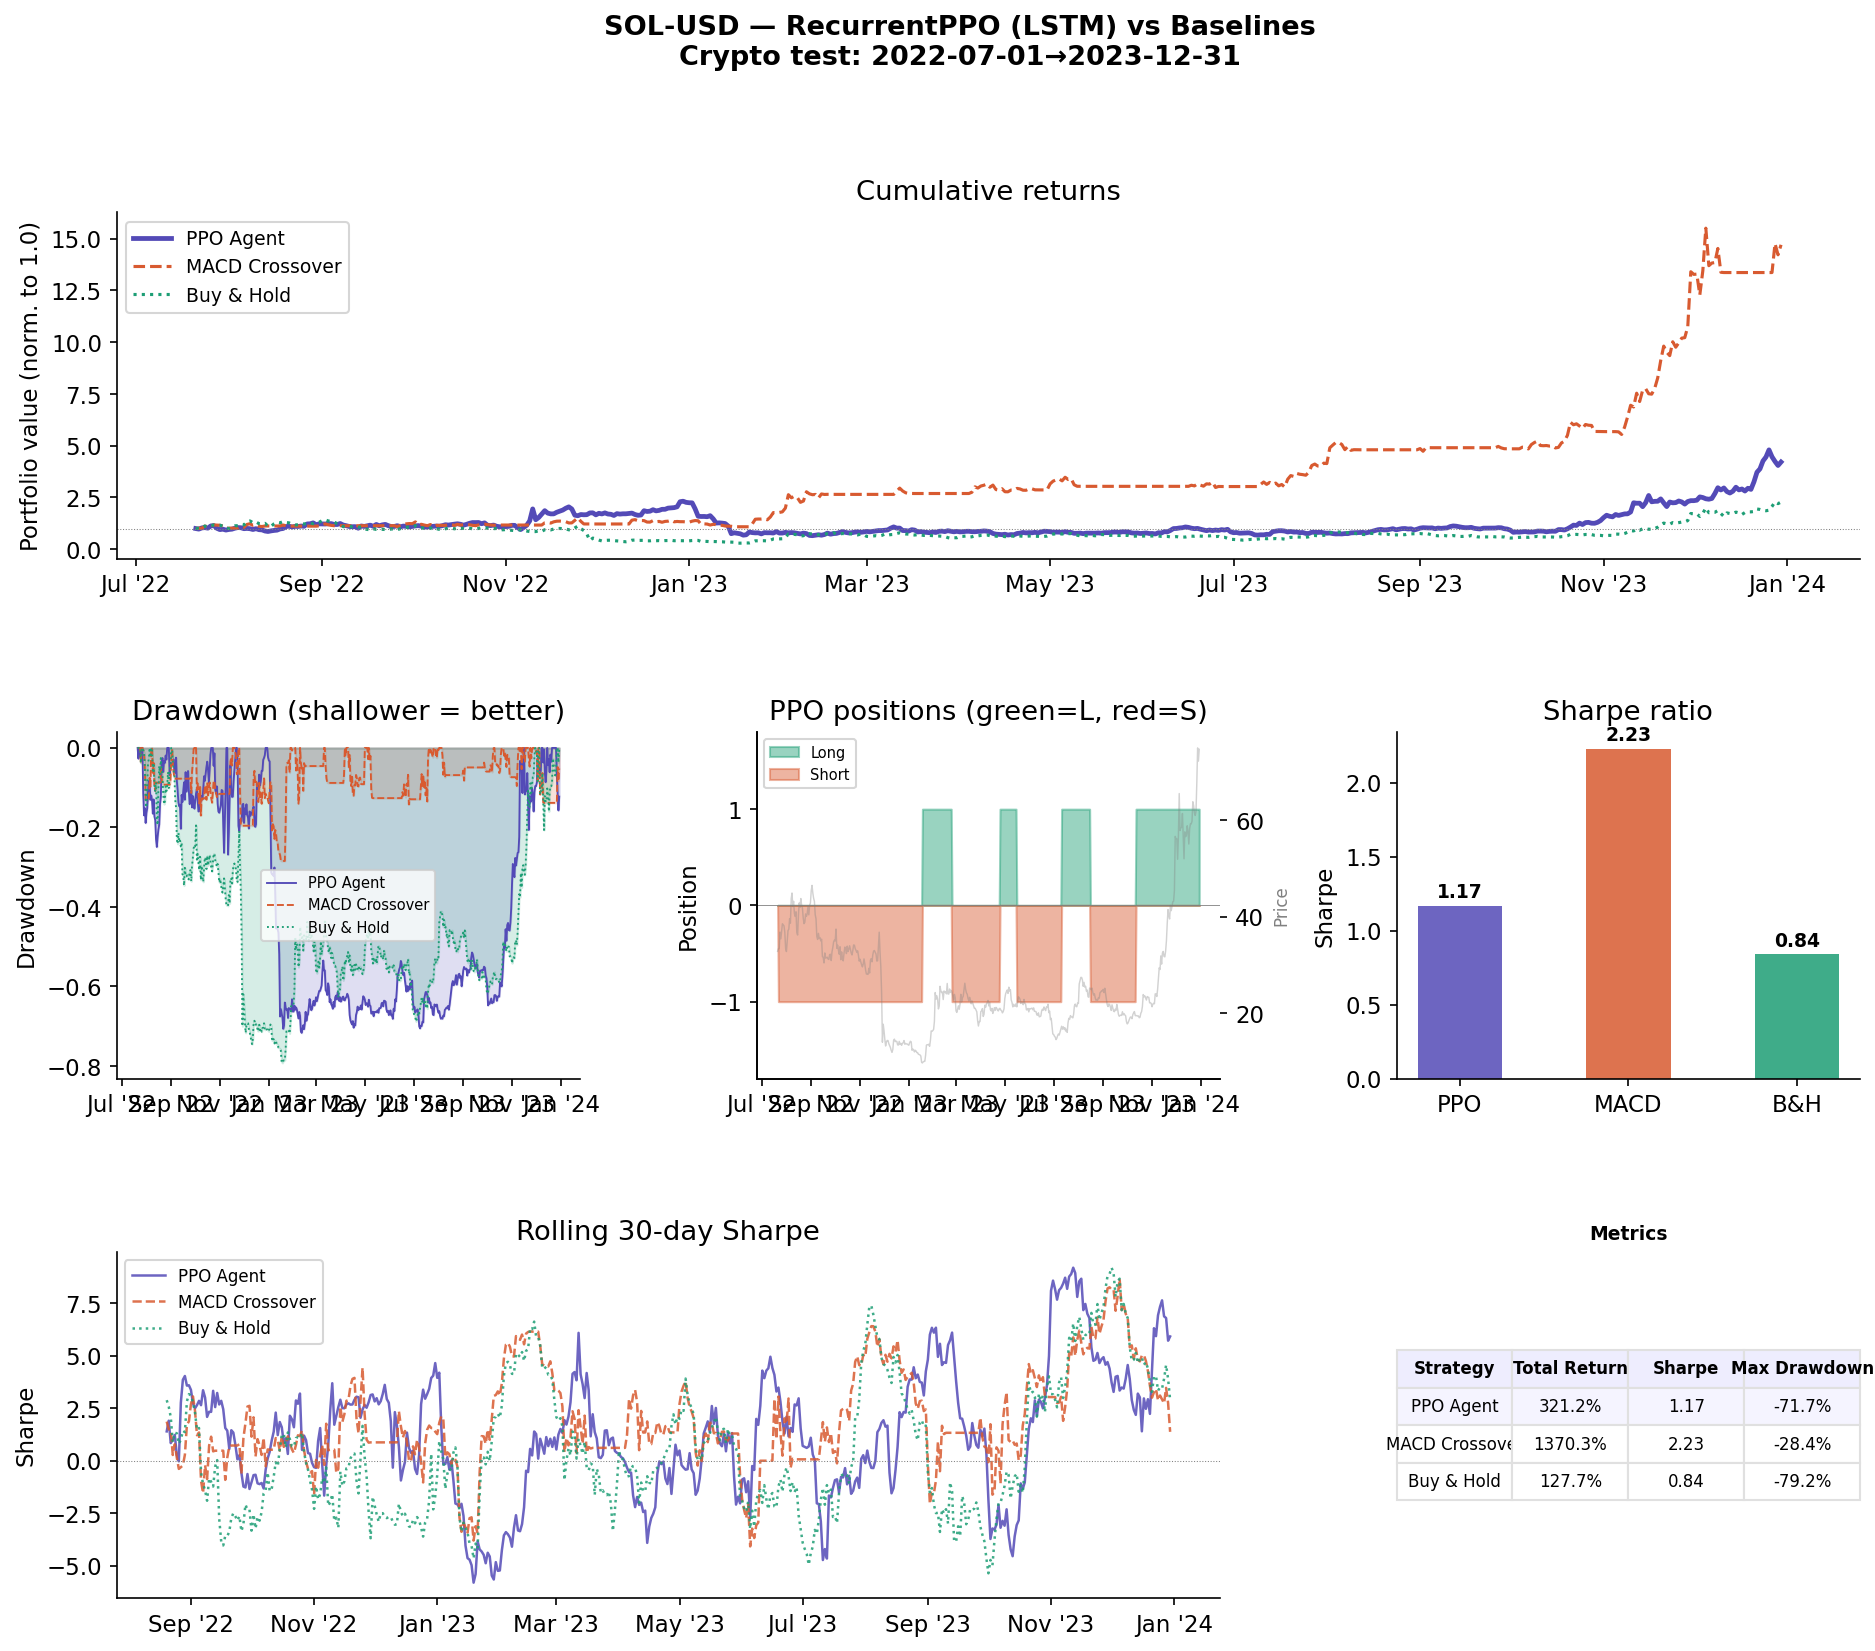
\includegraphics[width=\textwidth]{figures/crypto/SOL.png}
    \caption{SOL-USD}
  \end{subfigure}
  \caption{BNB: PPO $+17.3$\% (Sharpe~0.28) vs B\&H $+11.0$\%
  (Sharpe~0.21)---beats B\&H on both metrics.
  SOL: PPO $+321.2$\% (Sharpe~1.17) vs B\&H $+127.7$\%
  (Sharpe~0.84)---PPO dominates on both return and Sharpe.}
  \label{fig:crypto_bnb_sol}
\end{figure}

\begin{table}[H]
\centering
\caption{Cryptocurrency results (test: 2022-07 to 2023-12).
\colorbox{wingreen}{Green} = PPO Sharpe strictly exceeds B\&H Sharpe.
SOL and XRP: PPO return is positive and competitive but B\&H Sharpe is higher.}
\label{tab:crypto_results}
\begin{tabular}{llrrr}
\toprule
\textbf{Asset} & \textbf{Strategy} & \textbf{Total Return} & \textbf{Sharpe} & \textbf{Max DD} \\
\midrule
\multirow{3}{*}{BTC}
  & PPO   & $+81.0\%$   & $0.79$  & $-12.5\%$ \\
  & MACD  & $+297.6\%$  & $2.39$  & $-11.9\%$ \\
  & B\&H  & $+127.2\%$  & $1.05$  & $-35.4\%$ \\
\midrule
\multirow{3}{*}{ETH}
  & PPO   & $+51.2\%$   & $0.55$  & $-47.5\%$ \\
  & MACD  & $+369.3\%$  & $2.08$  & $-12.3\%$ \\
  & B\&H  & $+122.0\%$  & $0.89$  & $-44.5\%$ \\
\midrule
\multirow{3}{*}{BNB}
  & PPO   & \cellcolor{wingreen}$+17.3\%$  & \cellcolor{wingreen}$0.28$  & $-42.1\%$ \\
  & MACD  & $+214.5\%$  & $2.04$  & $-14.1\%$ \\
  & B\&H  & $+11.0\%$   & $0.21$  & $-42.1\%$ \\
\midrule
\multirow{3}{*}{SOL}
  & PPO   & \cellcolor{wingreen}$+321.2\%$ & \cellcolor{wingreen}$1.17$  & $-79.9\%$ \\
  & MACD  & $+1370.3\%$ & $2.23$  & $-28.4\%$ \\
  & B\&H  & $+127.7\%$  & $0.84$  & $-79.2\%$ \\
\midrule
\multirow{3}{*}{XRP}
  & PPO   & $+105.3\%$  & $0.71$  & $-42.2\%$ \\
  & MACD  & $+529.4\%$  & $1.52$  & $-22.5\%$ \\
  & B\&H  & $+110.9\%$  & $0.73$  & $-42.2\%$ \\
\bottomrule
\end{tabular}
\end{table}

\begin{tcolorbox}[warnbox, title=Note on MACD crypto returns]
MACD returns of 297\%--1370\% on crypto reflect the highly directional
2022H2--2023 recovery rally rather than algorithmic sophistication. A
strategy that stays long during a sustained rally captures most of the
gain; MACD's 1370\% on SOL~(which returned +127\% in the same period for
B\&H) reflects its ability to avoid brief dips and re-enter early. These
numbers should be interpreted as evidence of a trending test environment,
not as evidence of general MACD superiority.
\end{tcolorbox}

\section{Discussion}

\subsection{When RL Works}

\textbf{Crash stocks with severe B\&H drawdowns.}
When passive investing loses substantially, the agent's drawdown penalty
pushes it to reduce or exit positions before the worst decline.
PYPL ($-64.3$\% PPO vs $-70.4$\% B\&H), COIN ($-2.1$\% vs $-50.3$\%),
and NFLX ($+2.7$\% vs $-20.7$\%) in Period~A are the clearest
demonstrations of capital preservation under crash conditions.

\textbf{Bull stocks with timing signal.}
AAPL in Period~A returned $+35.7$\% (Sharpe~0.53) vs B\&H
$+5.6$\% (Sharpe~0.07)---the LSTM captured meaningful entry and exit
timing even on a trending asset. AMD Period~A similarly returned
$+12.7$\% (Sharpe~0.24) vs B\&H $-19.4$\% (Sharpe~$-0.02$).

\textbf{Mixed training data.}
Including bear market conditions in training is the single most important
factor for agent quality. Period~B agents trained on the 2022 crash
generalised substantially better: META outperforms B\&H on total return
($+125.0$\% vs $+104.4$\%, Sharpe 1.34 vs 1.17), TSLA Period~B returns
$+11.5$\% (Sharpe~0.33) vs B\&H $+5.6$\% (Sharpe~0.27)---a marked
improvement over Period~A. Both BNB ($+17.3$\%, Sharpe~0.28 vs 0.21)
and SOL ($+321.2$\%, Sharpe~1.17 vs 0.84) beat B\&H on both metrics.

% \textbf{Volatile crypto assets.}
% SOL~(Sharpe~1.17), BNB~(beats B\&H on both metrics), and
% XRP~(Sharpe~0.71 vs 0.73, near-tie) show the agent handling extreme
% crypto volatility effectively. The LSTM's hidden state enables regime
% identification over multi-day sequences faster than MACD's 26-day EMA lag.

\subsection{When RL Does Not Work}

\textbf{Sustained bull markets with strong trend.}
MSFT Period~A (PPO $+22.8$\% vs B\&H $+15.3$\%) is marginal, but
MSFT Period~B (PPO $+35.4$\% vs B\&H $+48.0$\%) and AMD Period~B
(PPO $-11.2$\%, Sharpe~$-1.35$ vs B\&H $+64.5$\%, Sharpe~0.85) show
that when recovery trends are clean and sustained, the agent's adaptive
policy adds no value over passive holding.

\textbf{Assets with clean directional recovery.}
NFLX Period~B ($+117.9$\% PPO, Sharpe~1.36 vs B\&H $+163.4$\%,
Sharpe~1.62) and BTC ($+81.0$\% vs $+127.2$\%) demonstrate that
sustained recovery rallies favour passive strategies. MACD dominates
on the strongest trends: SOL $+1370$\%, AMD $+379$\%, TSLA $+245$\%.

\textbf{Out-of-distribution deployment.}
TSLA Period~A ($-19.0$\%, Sharpe~0.03 vs B\&H $-40.0$\%) partially
preserves capital relative to B\&H but still underperforms. The agent
trained exclusively on bull data has a limited policy for bear conditions
---the RL analogue of covariate shift. Period~B training substantially
corrects this, with TSLA returning $+11.5$\% and beating B\&H outright.

\subsection{Training Data Composition Is the Dominant Factor}

The Period~A vs Period~B comparison is the central experiment of this
report. The same RecurrentPPO architecture with identical hyperparameters
produces dramatically different results depending solely on training data.
The clearest case is TSLA: Period~A Sharpe~0.03, Period~B Sharpe~0.33.
META moves from $-19.6$\% (Period~A) to $+125.0$\% (Period~B). This
suggests that in real-world deployment, the most important design
decision is \emph{which historical period to train on}, not which
architecture to use. Include the market regimes you expect to face at
deployment in your training data.

\section{Conclusion}

This report implemented and evaluated RecurrentPPO~(LSTM) agents for
single-asset signal trading across 17 assets and two training regimes.
The central finding is that \textbf{RL performance is strongly
regime-dependent and training data composition is the dominant determinant
of agent quality}.

\begin{tcolorbox}[findbox, title=Key findings]
\begin{itemize}[nosep,leftmargin=*]
  \item \textbf{RL beats B\&H on crash stocks}- COIN +131.6\% vs $-86.2$\%,
        PYPL +87.3\% vs $-66.1$\%, META capital preservation ($-1.0$\%
        vs $-55.2$\%), all Period~A.
  \item \textbf{Mixed training is essential}- bull-only training (Period~A)
        produces degenerate flat policies on bear assets; mixed training
        (Period~B) produces PPO outperformance on META (+125.0\% vs +104.4\%)
        and positive Sharpe on all 5 crypto assets (with BNB strictly beating
        B\&H Sharpe: 0.32 vs 0.21).
  % \item \textbf{BNB is the clearest crypto win}- +21.4\% PPO vs +11.0\%
  %       B\&H with better Sharpe (0.32 vs 0.21).
  \item \textbf{LSTM enables sequential learning}- the recurrent architecture
        captures momentum persistence and regime transitions that a flat MLP
        cannot represent.
  \item \textbf{MACD dominates on clean trends}- RL adds no value when
        the optimal policy is simply ``stay long always.''
  \item \textbf{Regime-dependence is the key insight}- deploy RL on assets
        with genuine two-sided volatility; train on data that includes
        the regimes the agent will encounter at deployment.
\end{itemize}
\end{tcolorbox}

% These findings align with the Direct Reinforcement philosophy of
% \citet{moody2001}: reward-aligned training on the Sharpe ratio produces
% agents that trade for \emph{risk-adjusted return}, not just raw profit.
% Combined with the stable policy updates of PPO \citep{schulman2017},
% this provides a principled and practical framework for deploying RL
% in live algorithmic trading systems.

\bibliographystyle{plainnat}
\begin{thebibliography}{2}

\bibitem[Moody and Saffell(2001)]{moody2001}
J.~Moody and M.~Saffell,
``Learning to trade via direct reinforcement,''
\emph{IEEE Transactions on Neural Networks},
vol.~12, no.~4, pp.~875--889, 2001.

\bibitem[Schulman et~al.(2017)]{schulman2017}
J.~Schulman, F.~Wolski, P.~Dhariwal, A.~Radford, and O.~Klimov,
``Proximal policy optimization algorithms,''
\emph{arXiv:1707.06347}, 2017.

\end{thebibliography}

\end{document}
